\documentclass[12pt, a4paper]{article}
\usepackage[margin=0.5in]{geometry}

\usepackage{color}
\usepackage[dvipsnames]{xcolor}
\usepackage{hyperref}
\hypersetup{
    colorlinks=true,
    linkcolor=blue,
    urlcolor=blue,
    linktoc=all
}


\usepackage{amsmath}
\usepackage{mathtools}
\usepackage{amssymb}
\usepackage{cancel}
\usepackage{bm}
\usepackage{dsfont}
\usepackage{graphicx}
\usepackage{graphics}
\usepackage{xfrac}
\usepackage{array}
\setcounter{MaxMatrixCols}{40}

\usepackage{enumerate}
\usepackage{enumitem}
\usepackage{multirow}

%inclusions carried over from past class homework formats
\usepackage{units}
\usepackage{fullpage}
\usepackage{alltt}
\usepackage{mathrsfs}
\usepackage{xcolor}
\usepackage{soul}

\usepackage{pgfplots}

\DeclarePairedDelimiter{\abs}{\lvert}{\rvert}
\newcommand*{\fontCourier}{\fontfamily{pcr}\selectfont}
\newcommand*\mean[1]{\overline{#1}}
\newcommand\scalemath[2]{\scalebox{#1}{\mbox{\ensuremath{\displaystyle #2}}}}

\setcounter{tocdepth}{5}
\setcounter{secnumdepth}{5}

\usepackage{pdfpages}
\usepackage{Sweave}
\begin{document}
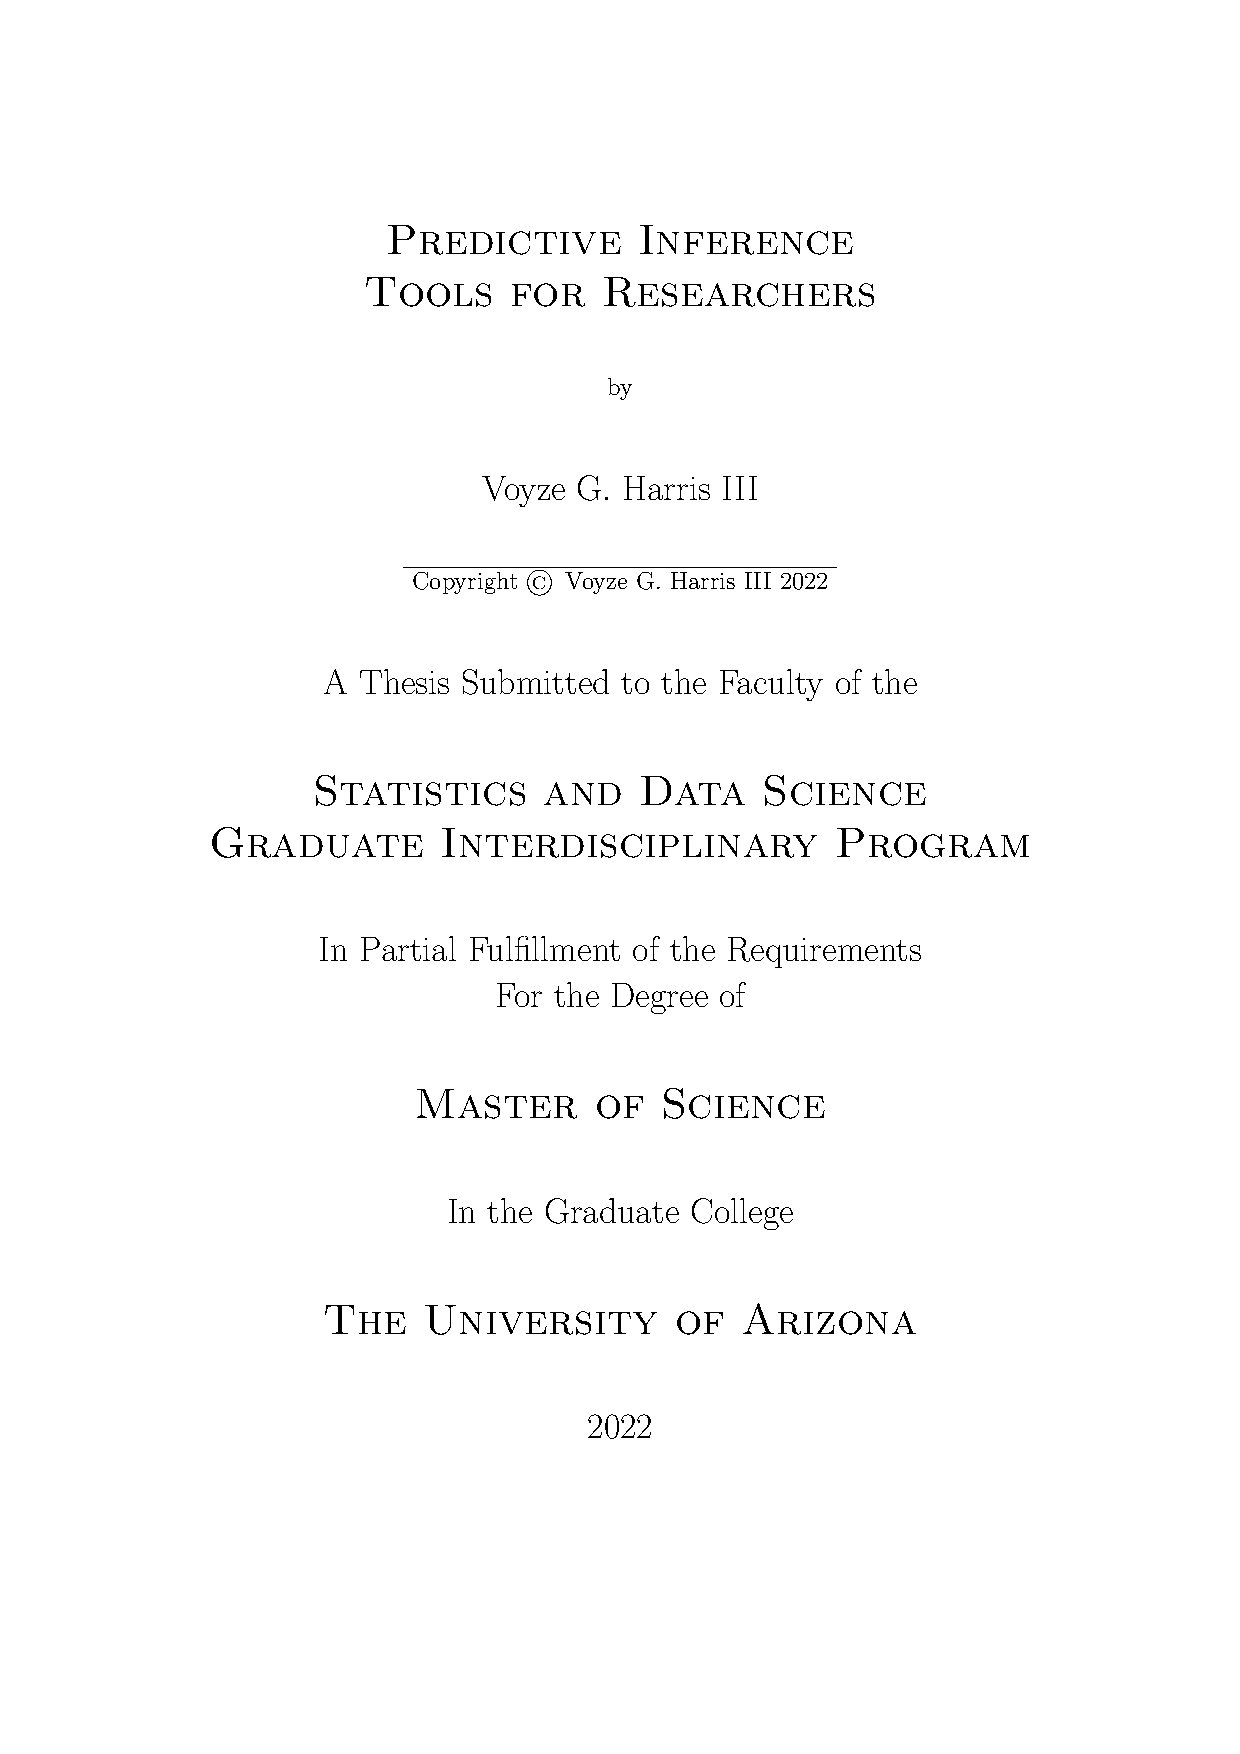
\includepdf{TitlePage_MastersThesis}

\includepdf{ThesisApprovalPage}
\Sconcordance{concordance:Thesis.tex:Thesis.Rnw:%
1 49 1 1 0 7 1 1 4 99 1 1 31 1 12 69 1 1 45 1 2 179 1 1 46 1 2 120 1 1 %
23 7 0 1 76 4 0 1 5 32 1 1 26 1 4 26 1}


\tableofcontents
\newpage


%%%%%%%%%%%%%%%%%%%%%%%%%%%%%%%%%
%%INTRODUCTION
%%%%%%%%%%%%%%%%%%%%%%%%%%%%%%%%%
\section{Thesis Abstract}
  \begin{itemize}
    \item (paragraph) Statement of the thesis topic and objectives
    \item (paragraph) Explanation of R package
  \end{itemize}

\clearpage

\section{Introduction:  Predictive Inference}

  \subsection{Why is predictive inference important?}

  \subsection{Difference between parametric inference and predictive inference}

    \subsubsection{When is predictive inference more useful?}

    \subsubsection{When is parametric inference more useful?}
      [examples, comparisons]

  \subsection{The Bayesian Parametric Prediction Format}
    [Geisser p. 49]\\

        Let $$f\left(x^{(N)},x_{(M)}|\theta\right) = f\left(x_{(M)}|x^{(N)},\theta\right)f\left(x^{(N)}|\theta\right).$$

    Here $x^{(N)}$ represents observed events and $x_{(M)}$ are future events.  We calculate

    $$f\left(x_{(M)},x^{(N)}\right) = \int f\left(x^{(N)},x_{(M)}|\theta\right)p(\theta)d\theta$$

    where $p(\theta)$ is the prior density and

    $$f\left(x_{(M)}|x^{(N)}\right) = \frac{f\left(x_{(M)},x^{(N)}\right)}{f\left(x^{(N)}\right)} = \int f\left(x_{(M)}|\theta\right)p\left(\theta|x^{(N)}\right)d\theta$$

    where

    $$p\left(\theta|x^{(N)}\right) \propto f\left(x^{(N)}|\theta\right)p(\theta).$$

  \subsection{[Maybe] Example of Difference between results from Plug-in estimator and results using Predictive Inference}

\clearpage

\section{Chapter 1:  Predictive Problems with Conjugate Priors}

  [Problems with closed-form solutions.  These problems will be what the R package is designed for.  Use problems from Geisser, Casella \& Berger (Bayesian chapter), other sources.  Regression problem--predictive distributions of models that include and exclude some predictor]

  \subsection{Prediction of Future Successes:  Beta-Binomial (Geisser p. 73)}


    \subsubsection{Derivation}

      Let $X_i$ be independent binary variables with Pr$(X_i = 1) = \theta$, and let $T = \sum X_i$.  Then $T$ has probability

      $${N\choose t}\theta^t(1-\theta)^{N-t}.$$

      \vspace{5mm}

      Assume $\theta\sim\text{Beta}(\alpha,\beta)$, so

      \vspace{5mm}

      $$p(\theta) = \frac{\Gamma(\alpha + \beta)\theta^{\alpha - 1}(1 - \theta)^{\beta - 1}}{\Gamma(\alpha)\Gamma(\beta)}.$$

      \vspace{5mm}

      Then

      \vspace{5mm}

      $$p\left(\theta|X^{(N)}\right) = \frac{\Gamma(N+\alpha+\beta)\theta^{t+\alpha-1}(1-\theta)^{N-t+\beta-1}}{\Gamma(t+\alpha)\Gamma(N-t+\beta)}$$

      \vspace{5mm}

      \noindent So for $R = \sum_{i=1}^M X_{N+i}$ we have Beta-Binomial predictive distribution

\begin{flalign*}
  \text{Pr}[R=r|t]
  &= \int {M\choose r}\theta^r(1-\theta)^{M-r}p\left(\theta|X^{(N)}\right)d\theta\\
  &\\
  &= {M\choose r}\int \theta^r(1-\theta)^{M-r}\frac{\Gamma(N+\alpha+\beta)}{\Gamma(t+\alpha)\Gamma(N-t+\beta)}\theta^{t+\alpha-1}(1-\theta)^{N-t+\beta-1}d\theta\\
  &\\
  &= \frac{M!}{r!(M-r)!}\frac{\Gamma(N+\alpha+\beta)}{\Gamma(t+\alpha)\Gamma(N-t+\beta)}\int\theta^{r+t+\alpha-1}(1-\theta)^{M-r+N-t+\beta-1}d\theta\\
  &\\
  &= \frac{\Gamma(M+1)\Gamma(N+\alpha+\beta)\Gamma(r+t+\alpha)\Gamma(M-r+N-t+\beta)}{\Gamma(r+1)\Gamma(M-r+1)\Gamma(t+\alpha)\Gamma(N-t+\beta)\Gamma(M+N+\alpha+\beta)}
\end{flalign*}

\clearpage

    \subsubsection{R Implementation}

This result has been used to create ``standard" R functions dpredBB(), ppredBB(), and rpredBB() for the Beta-Binomial distribtuion for density, cumulative probability, and random sampling, respectively (see appendix).  These functions are exercised in the following example.


    \subsubsection{Example}

Suppose $t=5$ successes have been observed out of $N=10$ binary events, $\alpha = 2$ and $\beta = 8$.  For $M = 1000$ future observations, the figures below show the predictive distribution from dpredBB(), the cumulative distribution from ppredBB(), and a histogram of random draws from rpredBB().


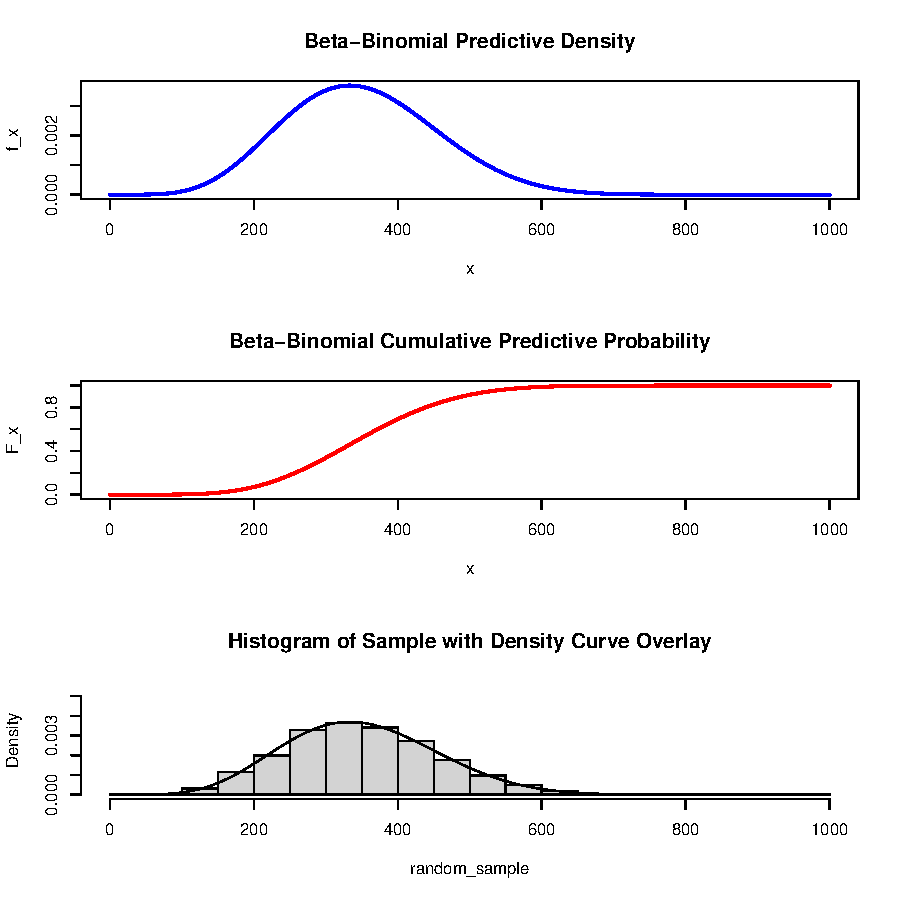
\includegraphics{Thesis-002}



    \subsection{Survival Time:  Exponential-Gamma (Geisser p. 74)}


    \subsubsection{Derivation}

      Suppose $X^{(N)} = \left(X^{(d)},X^{(N-d)}\right)$ where $X^{(d)}$ represents copies fully observed from an exponential survival time density
          $$f(x|\theta) = \theta e^{-\theta x}$$
      and $X^{(N-d)}$ represents copies censored at $x_{d+1},...,x_N$, respectively.  Hence
          $$L(\theta)\propto\theta^d e^{-\theta N\bar{x}}$$
      when $N\bar{x} = \sum_1^N{x_i}$, as shown below.\\

      The usual exponential likelihood is used for the fully observed copies, whereas for the censored copies we need Pr$(x > \theta) = 1 - \text{Pr}(x\leq\theta) = 1 - F(x|\theta) = 1 - (1 - e^{-\theta x}) = e^{-\theta x}$.  Thus the overall likelihood is

      $$L(\theta|x) = \prod_{i=1}^d\theta e^{-\theta x_i}\prod_{i=d+1}^N e^{-\theta x_i} = \theta^d e^{-\theta N\bar{x}}$$

      Assuming a Gamma$(\delta,\gamma)$ prior for $\theta$,

       $$p(\theta) = \frac{\gamma^\delta\theta^{\delta - 1}e^{-\gamma\theta}}{\Gamma(\delta)}$$

       we obtain the posterior

       %$$p\left(\theta|X^{(N)}\right) = \frac{p\left(x^{(N)}|\theta\right)p(\theta)}{\int p\left(X^{(N)}|\theta\right)p(\theta)d\theta} = \frac{(\gamma+N\bar{x})^{d+\delta}\theta^{d+\delta - 1}e^{-\theta(\gamma+N\bar{x})}}{\Gamma(d+\delta)}$$

        \begin{flalign*}
          p\left(\theta|X^{(N)}\right)
          &= \frac{p\left(x^{(N)}|\theta\right)p(\theta)}{\int p\left(X^{(N)}|\theta\right)p(\theta)d\theta}\\
          &\\
          &= \frac{\theta^d e^{-\theta N\bar{x}}\cdot\frac{\gamma^\delta\theta^{\delta - 1}e^{-\gamma\theta}}{\Gamma(\delta)}}{\int\left(\theta^d e^{-\theta N\bar{x}}\cdot\frac{\gamma^\delta\theta^{\delta - 1}e^{-\gamma\theta}}{\Gamma(\delta)}\right)d\theta}\\
          &\\
          &= \frac{\cancel{\frac{\gamma^\delta}{\Gamma(\delta)}}\left(\theta^{d+\delta - 1}e^{-\theta(\gamma+N\bar{x})}\right)}{\cancel{\frac{\gamma^\delta}{\Gamma(\delta)}}\int\left(\theta^{d+\delta - 1}e^{-\theta(\gamma+N\bar{x})}\right)d\theta}\\
          &\\
          &= \frac{\frac{(\gamma+N\bar{x})^{d+\delta}}{\Gamma(d+\delta)}\left(\theta^{d+\delta - 1}e^{-\theta(\gamma+N\bar{x})}\right)}{\cancel{\frac{(\gamma+N\bar{x})^{d+\delta}}{\Gamma(d+\delta)}\int\left(\theta^{d+\delta - 1}e^{-\theta(\gamma+N\bar{x})}\right)d\theta}}\\
          &\\
          &= \frac{(\gamma+N\bar{x})^{d+\delta}\theta^{d+\delta - 1}e^{-\theta(\gamma+N\bar{x})}}{\Gamma(d+\delta)}
        \end{flalign*}

    with the Gamma$(d+\delta,\gamma+N\bar{x})$ density in the next to last step integrating to $1$.\\

    Thus the survival time predictive probability is

    \begin{flalign*}
      P\left(X = x|\theta,X^{(N)}\right)
      &= \int p\left(\theta|X^{(N)}\right)p(x|\theta)d\theta\\
      &\\
      &= \int\frac{(\gamma+N\bar{x})^{d+\delta}\theta^{d+\delta - 1}e^{-\theta(\gamma+N\bar{x})}}{\Gamma(d+\delta)}\cdot\theta e^{-\theta x}d\theta\\
      &\\
      &= (d+\delta)(\gamma+N\bar{x})^{d+\delta}\int\frac{\theta^{(d+\delta + 1) - 1}e^{-\theta(\gamma+N\bar{x} + x)}}{(d+\delta)\Gamma(d+\delta)}d\theta\\
      &\\
      &= \frac{(d+\delta)(\gamma+N\bar{x})^{d+\delta}}{\left(\gamma+N\bar{x}+x\right)^{d+\delta+1}}\int\frac{\left(\gamma+N\bar{x}+x\right)^{d+\delta+1}\theta^{(d+\delta + 1) - 1}e^{-\theta(\gamma+N\bar{x} + x)}}{\Gamma(d+\delta+1)}d\theta\\
      &\\
      &= \frac{(d+\delta)(\gamma+N\bar{x})^{d+\delta}}{\left(\gamma+N\bar{x}+x\right)^{d+\delta+1}}
    \end{flalign*}

    (simplifying by constructing a Gamma$(d+\delta+1,\gamma+N\bar{x}+x)$ density in the final integrand.)\\



    \subsubsection{R Implementation}

This result has been used to create standard format R functions dpredEG(), ppredEG(), and rpredEG() for the Gamma-Exponential distribtuion for density, cumulative probability, and random sampling, respectively (see appendix).  These functions are exercised in the following example.


    \subsubsection{Example}

Suppose $d=800$ out of $N = 1000$ copies have been observed, and the remaining $200$ censored.  Say $\delta = 20$, $\gamma=5$, and we are interested in the number of survivors out of $M = 1000$ future observations.  The figures below illustrate the predictive probability using dpredEG() and rpredEG(), along with a histogram of a random sample taken using rpredEG().


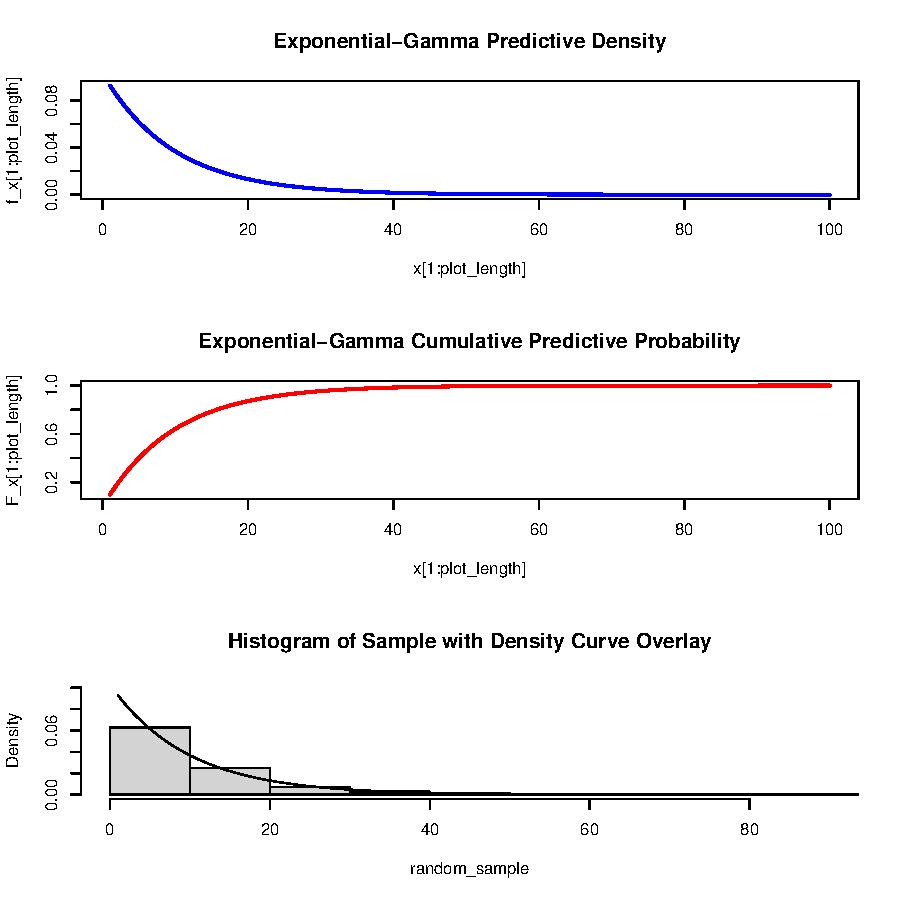
\includegraphics{Thesis-003}

\clearpage

  \subsection{Poisson-Gamma Model (Hoff p. 43ff)}
    \subsubsection{Derivation}
    [using Hoff's notation and variable names below.  Should I convert this to Geisser's $x^{(N)},x_{(M)}$ convention for uniformity throughout my thesis?]\\\\
      Suppose $Y_1,...,Y_n|\theta\overset{i.i.d.}{\sim}\text{Poisson}(\theta)$ with Gamma prior $\theta\sim\text{Gamma}(\alpha,\beta)$.  That is,

      \begin{flalign*}
        P\left(Y_1 = y_1,...,Y_n = y_n|\theta\right)
        &= \prod_{i=1}^n p\left(y_i|\theta\right)\\
        &\\
        &= \prod_{i=1}^n\frac{1}{y!}\theta^{y_i}e^{-\theta}\\
        &\\
        &= \left(\prod_{i=1}^n\frac{1}{y!}\right)\theta^{\sum y_i}e^{-n\theta}\\
        &\\
        &= c\left(y_1,...,y_n\right)\theta^{\sum y_i}e^{-n\theta}
      \end{flalign*}

      and

      $$p(\theta) = \dfrac{\beta^\alpha}{\Gamma(\alpha)}\theta^{\alpha-1}e^{-\beta\theta}, \theta, \alpha, \beta > 0.$$

\bigskip

      Then we have posterior distribution

      \begin{flalign*}
        p\left(\theta|y_1,...,y_n\right)
        &= \dfrac{p\left(y_1,...,y_n|\theta\right)p(\theta)}{\int_\theta p\left(y_1,...,y_n|\theta\right)p(\theta)}\\
        &\\
        &= \dfrac{p\left(y_1,...,y_n|\theta\right)p(\theta)}{p\left(y_1,...,y_n\right)}\\
        &\\
        &= \dfrac{1}{p\left(y_1,...,y_n\right)}\theta^{\sum y_i}e^{-n\theta}\dfrac{\beta^\alpha}{\Gamma(\alpha)}\theta^{\alpha - 1}e^{-\beta\theta}\\
        &\\
        &= C\left(y_1,...,y_n,\alpha,\beta\right)\theta^{\alpha+\sum y_i - 1}e^{-(\beta + n)\theta}\\
        &\\
        &\sim \text{Gamma}\left(\alpha+\sum y_i,\beta + n\right).
      \end{flalign*}


      Here

      \begin{flalign*}
        C\left(y_1,...,y_n,\alpha,\beta\right)
        &= \dfrac{1}{p\left(y_1,...,y_n\right)}\cdot\dfrac{\beta^\alpha}{\Gamma(\alpha)}\\
        &\\
        &= \dfrac{1}{\int_\theta p\left(y_1,...,y_n|\theta\right)p(\theta)}\cdot\dfrac{\beta^\alpha}{\Gamma(\alpha)}\\
        &\\
        &= \dfrac{1}{\int_\theta\left(\prod\frac{1}{y_i!}\right)\theta^{\sum y_i}e^{-n\theta}\cancel{\left(\frac{\beta^\alpha}{\Gamma(\alpha)}\right)}\theta^{\alpha-1}e^{-\beta\theta}}\cdot\cancel{\left(\frac{\beta^\alpha}{\Gamma(\alpha)}\right)}
        &\\
        &= \dfrac{1}{\left(\prod\frac{1}{y_i!}\right)\frac{\Gamma(\alpha + \sum y_i)}{(\beta+n)^{\alpha+\sum y_i}}\int_\theta \frac{(\beta+n)^{\alpha+\sum y_i}}{\Gamma(\alpha+\sum y_i)}\theta^{\sum y_i+\alpha-1}e^{-(\beta+n)\theta}}\\
        &\\
        &= \dfrac{\prod_{i=1}^n y_i!(\beta+n)^{\alpha+\sum y_i}}{\Gamma(\alpha+\sum y_i)}
      \end{flalign*}

      Call this constant $C_n$ (for $n$ observations).

\bigskip

      Note that an additional observation $y_{n+1} = \tilde{y}$ the constant becomes

      $$C_{n+1} = \dfrac{\prod_{i=1}^{n+1} y_i!(\beta+n+1)^{\alpha+\sum_{i=1}^{n+1} y_i}}{\Gamma(\alpha+\sum_{i=1}^{n+1} y_i)}.$$

      Also note that the marginal joint distribution of $k$ observations is

      $$p\left(\tilde{y}|y_1,...,y_k\right) = \dfrac{1}{C_k}\dfrac{\beta^\alpha}{\Gamma(\alpha)}.$$

      For future observation $\tilde{y}$, then, we compute predictive distribution

      \begin{flalign*}
        p\left(\tilde{y}|y_1,...,y_n\right)
        &= \dfrac{p\left(y_1,...,y_n,\tilde{y}\right)}{p\left(y_1,...,y_n\right)} = \dfrac{p\left(y_1,...,y_{n+1}\right)}{p\left(y_1,...,y_n\right)}
        = \dfrac{\frac{1}{C_{n+1}}\cancel{\frac{\beta^\alpha}{\Gamma(\alpha)}}}{\frac{1}{C_n}\cancel{\frac{\beta^\alpha}{\Gamma(\alpha)}}}
        = \dfrac{C_n}{C_{n+1}}\\
        &\\
        &= \dfrac{\dfrac{\prod_{i=1}^n y_i!(\beta+n)^{\alpha+\sum_{i=1}^n y_i}}{\Gamma(\alpha+\sum_{i=1}^n y_i)}}{\dfrac{\prod_{i=1}^{n+1} y_i!(\beta+n+1)^{\alpha+\sum_{i=1}^{n+1} y_i}}{\Gamma(\alpha+\sum_{i=1}^{n+1} y_i)}}\\
        &\\
        &= \dfrac{\Gamma\left(\alpha+\sum_{i=1}^{n+1}y_i\right)(\beta+n)^{\alpha+\sum_{i=1}^n y_i}}{\left(y_{n+1}!\right)\Gamma\left(\alpha+\sum_{i=1}^n y_i\right)(\beta+n+1)^{\alpha+\sum_{i=1}^{n+1}y_i}}\\
        &\\
        &= \dfrac{\Gamma\left(\alpha+\sum_{i=1}^n y_i + \tilde{y}\right)(\beta+n)^{\alpha+\sum_{i=1}^n y_i}}{\left(\tilde{y}!\right)\Gamma\left(\alpha+\sum_{i=1}^n y_i\right)(\beta+n+1)^{\alpha+\sum_{i=1}^n y_i + \tilde{y}}}\\
        &\\
        &= \dfrac{\Gamma\left(\alpha+\sum y_i+\tilde{y}\right)}{\Gamma(\tilde{y}+1)\Gamma(\alpha+\sum y_i)}\cdot \left(\dfrac{\beta+n}{\beta+n+1}\right)^{\alpha+\sum y_i} \cdot \left(\dfrac{1}{\beta+n+1}\right)^{\tilde{y}}\\
      \end{flalign*}

This is a negative binomial distribution:  $\tilde{y}\sim NB\left(\alpha+\sum y_i,\beta+n\right)$, for which

\begin{flalign*}
  E\left[\tilde{Y}|y_1,...,y_n\right] &= \dfrac{a+\sum{y_i}}{b+n} = E\left[\theta|y_1,...,y_n\right];\\
  &\\
  \text{Var}\left[\tilde{Y}|y_1,...,y_n\right] &= \dfrac{a+\sum{y_i}}{b+n}\dfrac{b+n+1}{b+n}\\
  &\\
  &=\text{Var}\left[\theta|y_1,...,y_n\right]\times(b+n+1)\\
  &\\
  &=E\left[\theta|y_1,...,y_n\right]\times\dfrac{b+n+1}{b+n}\\
\end{flalign*}

\vspace{5mm}

\hrule

\vspace{5mm}

[Showing here that it is indeed a NB distribution]

$$\theta\sim NB(\alpha,\beta)\Rightarrow p(\theta) = \binom{\theta+\alpha-1}{\alpha - 1}\left(\dfrac{\beta}{\beta+1}\right)^\alpha\left(\dfrac{1}{\beta+1}\right)^\theta$$

\begin{center}so\end{center}

\begin{flalign*}
  \tilde{y}\sim NB\left(\alpha + \sum{y_i}),\beta+n\right)\Rightarrow p(\tilde{y})
  &= \binom{\tilde{y}+\alpha+\sum{y_i}-1}{\alpha+\sum{y_i}-1}\left(\dfrac{\beta+n}{\beta+n+1}\right)^{\alpha+\sum{y_i}}\left(\dfrac{1}{\beta+n+1}\right)^{\tilde{y}}\\
  &\\
  &= \dfrac{\left(\alpha + \sum{y_i} + \tilde{y} - 1\right)!}{\left(\alpha + \sum{y_i} - 1\right)!\left(\tilde{y}\right)!}\left(\dfrac{\beta+n}{\beta+n+1}\right)^{\alpha+\sum{y_i}}\left(\dfrac{1}{\beta+n+1}\right)^{\tilde{y}}\\
  &\\
  &= \dfrac{\Gamma\left(\alpha + \sum{y_i} + \tilde{y}\right)}{\Gamma\left(\alpha + \sum{y_i}\right)\Gamma\left(\tilde{y}+1\right)}\left(\dfrac{\beta+n}{\beta+n+1}\right)^{\alpha+\sum{y_i}}\left(\dfrac{1}{\beta+n+1}\right)^{\tilde{y}}
\end{flalign*}

\vspace{5mm}

\hrule

\vspace{5mm}

      \bigskip



      [This is the result in Hoff.  The straightforward derivation below is off by a constant multiple.  Need to figure out what went awry.]



      \begin{flalign*}
        p\left(\tilde{y}|y_1,...,y_n\right)
        &= \int_0^\infty p\left(\tilde{y}|\theta,y_1,...,y_n\right)p\left(\theta|y_1,...,y_n\right)d\theta\\
        &\\
        &= \int p\left(\tilde{y}|\theta\right)p\left(\theta|y_1,...,y_n\right)d\theta\\
        &\\
        &= C\int\left(\dfrac{1}{\tilde{y}!}\theta^{\tilde{y}}e^{-\theta}\right)\theta^{\alpha+\sum y_i - 1}e^{-(\beta+n)\theta}d\theta\\
        &\\
        &= \dfrac{C}{\tilde{y}!}\int\theta^{\tilde{y}+\alpha+\sum y_i - 1}e^{-(\beta+n+1)\theta}d\theta\\
        &\\
        &= \dfrac{C\Gamma\left(\tilde{y}+\alpha+\sum y_i\right)}{\Gamma\left(\tilde{y}+1\right)(\beta+n+1)^{\tilde{y}+\alpha+\sum y_i}}\int\dfrac{(\beta+n+1)^{\tilde{y}+\alpha+\sum y_i}}{\Gamma\left(\tilde{y}+\alpha+\sum y_i\right)}\theta^{\tilde{y}+\alpha+\sum y_i - 1}e^{-(\beta+n+1)\theta)}d\theta\\
        &\\
        &= C\cdot\dfrac{\Gamma\left(\tilde{y}+\alpha+\sum y_i\right)}{\Gamma\left(\tilde{y}+1\right)(\beta+n+1)^{\tilde{y}+\alpha+\sum y_i}}\\
        &\\
        &= \dfrac{\prod_{i=1}^n y_i!(\beta+n)^{\alpha+\sum y_i}}{\Gamma(\alpha+\sum y_i)}\cdot\dfrac{\Gamma\left(\tilde{y}+\alpha+\sum y_i\right)}{\Gamma\left(\tilde{y}+1\right)(\beta+n+1)^{\tilde{y}+\alpha+\sum y_i}}\\
        &\\
        &= \prod_{i=1}^n y_i! \cdot \dfrac{\Gamma\left(\tilde{y}+\alpha+\sum y_i\right)}{\Gamma(\tilde{y}+1)\Gamma(\alpha+\sum y_i)}\cdot \left(\dfrac{\beta+n}{\beta+n+1}\right)^{\alpha+\sum y_i} \cdot \left(\dfrac{1}{\beta+n+1}\right)^{\tilde{y}}\\
      \end{flalign*}

\textcolor{red}{Hoff p.47:
  \begin{itemize}
    \item $b$ is interpreted as the number of prior observations
    \item $a$ is interpreted as the sum of counts from $b$ prior observations
  \end{itemize}
}

\textcolor{red}{  Hoff p. 49 (Birth rate example):  $a = 2, b = 1$. }


    \subsubsection{R Implementation}

This result has been used to create standard format R functions dpredPG(), ppredPG(), and rpredPG() for the Poisson-Gamma distribution for density, cumulative probability, and random sampling, respectively (see appendix).  These functions are exercised in the following example.\\

    Developing the random sample function rpredPG():  I need to establish the support of the predictive distribution $f_x$ from which to sample.  the uniroot() function is not working because it keeps feeding non-integer values to dnbinom().  Strategy: a modified bisection method as follows:\\

    \begin{enumerate}
      \item set a desired tolerance $\epsilon$.
      \item Find the expected value $E_x$ (closed formula, see above).
      \item Step to the right of $E_x$ by whole integers, in the sequence $E_x + \{1,2,4,...2^n\}$, stopping at $U=f_x\left(E_x + 2^n\right) < 0$.  This is the upper bound for the bisection method.
      \item Bisect the interval, rounding to the nearest integer.  Call the resulting mid-interval number $B$.
      \item If B is positive, test whether $0 \leq f_x(B) \leq \epsilon$.  If so, DONE.  If not:
      \item Establish new interval, choosing endpoints from $E_x$, $B$, and $U$ so that the interval straddles $0$, and repeat the steps until the condition in step 5 is reached.
    \end{enumerate}

    \subsubsection{Example}

Suppose we have 10 prior observations with counts 27, 79, 21, 100, 8, 4, 37, 15, 3, 97.  Let $\alpha = 11$ and $\beta = 3$.  For $\tilde{y} = 1:100$ possible future occurrences, the figures below show the predictive distribution from dpredPG(), the cumulative distribution from ppredPG(), and a histogram of random draws from rpredPG().

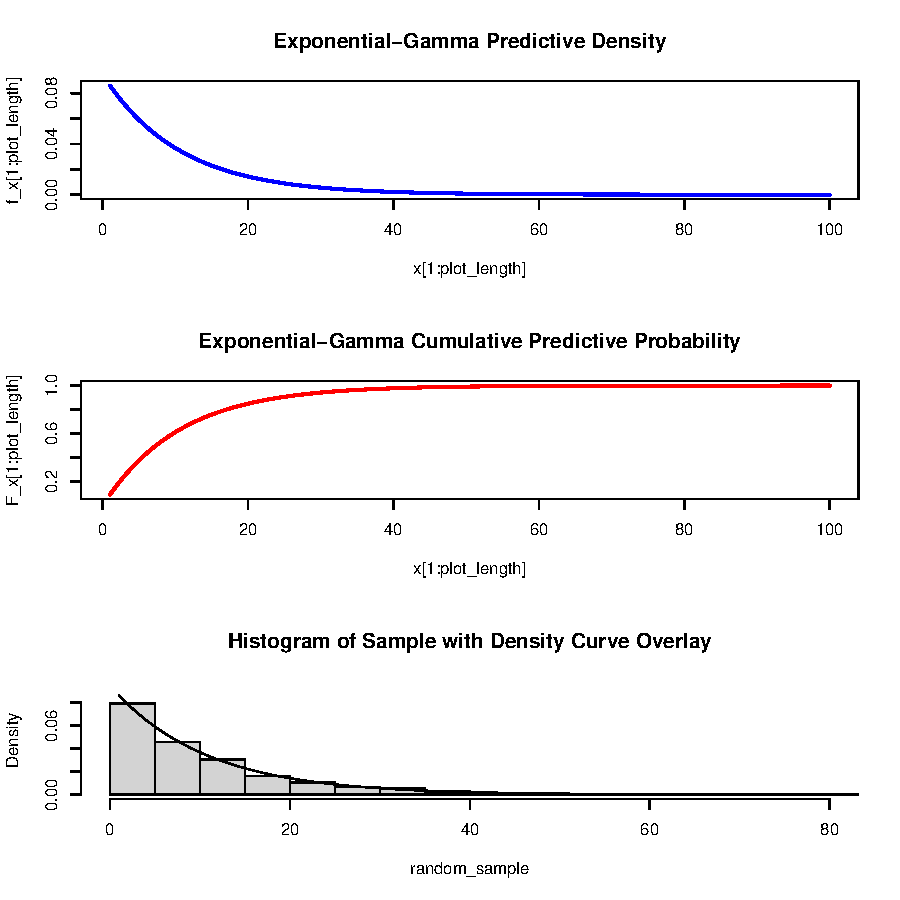
\includegraphics{Thesis-004}

\clearpage

  \subsection{Normal Observation with Normal-Inverse Gamma Prior}
    \subsubsection{One sample}
      \paragraph{Derivation}
      [Hoff p. 69ff]\\
        Let $\left\{Y_1,...,Y_n|\theta,\sigma^2\right\}\overset{i.i.d.}{\sim}N\left(\theta,\sigma^2\right)$.  Then the joint sampling density is

        \begin{flalign*}
          p\left(y_1,...,y_n|\theta,\sigma^2\right)
          &= \prod_{i=1}^n p\left(y_i|\theta,\sigma^2\right)\\
          &\\
          &= \prod_{i=1}^n \dfrac{1}{\sqrt{2\pi\sigma^2}}e^{-\frac{1}{2}\left(\frac{y_i - \theta}{\sigma}\right)^2}\\
          &\\
          &= \left(2\pi\sigma^2\right)^{-\sfrac{n}{2}}e^{-\frac{1}{2}\sum_{i=1}^n\left(\frac{y_i - \theta}{\sigma}\right)^2}.\\
        \end{flalign*}

        %It can be shown that $\left\{\sum{y_i^2},\sum{y_i}\right\}$ and hence $\left\{\bar{y},s^2\right\}$ are sufficient statistics, where $\bar{y} = \sum{y_i}/n$ and $s^2 = \sum\left(y_i - \bar{y}\right)^2/(n-1)$.\\


        %\vdots

        Following Hoff (p. 74ff), for joint inference on both $\theta$ and $\sigma$, assume priors

        \begin{flalign*}
          \frac{1}{\sigma^2} &\sim \text{gamma}\left(\sfrac{\nu_0}{2},\sfrac{\nu_0\sigma_0^2}{2}\right)\\
          &\\
          \theta|\sigma^2 &\sim \text{normal}\left(\mu_0,\sfrac{\sigma^2}{\kappa_0}\right)\\
        \end{flalign*}

        where $\left(\sigma_0^2,\nu_0\right)$ are the sample variance and sample size of prior observations, and $\left(\mu_o, \kappa_0\right)$ are the sample mean and sample size of prior observations.\\

        Note:  $\mu_0$, $\kappa_0$, $\nu_0$, and $\sigma_0^2$ come from prior knowledge. [in the Hoff example (Midge Wing Length), $\kappa_0$ and $\nu_0$ are both set to $1$ so that ``our prior distributions are only weakly centered around these estimates from other populations."]\\

        From this we derive joint posterior distribution

        \begin{flalign*}
          \left\{\theta|y_1,...,y_n,\sigma^2\right\} &\sim \text{normal}\left(\mu_n,\sfrac{\sigma^2}{\kappa_n}\right)\\
          &\\
          \left\{\sigma^2|y_1,...,y_n\right\} &\sim \text{inverse-gamma}\left(\sfrac{\nu_n}{2},\sfrac{\sigma^2_n\nu_n}{2}\right).
        \end{flalign*}

        where

        \begin{flalign*}
          \kappa_n &= \kappa_0 + n\\
          &\\
          \mu_n &= \frac{\kappa_0\mu_0+n\bar{y}}{\kappa_n}\\
          &\\
          \nu_n &= \nu_0 + n\\
          &\\
          \sigma_n^2 &= \frac{1}{\nu_n}\left[\nu_0\sigma_0^2 + (n-1)s^2 + \frac{\kappa_0 n}{\kappa_n}\left(\bar{y}-\mu_0\right)^2\right].\\
        \end{flalign*}

        Here $\bar{y} = \frac{1}{n}\sum_{i=1}^n y_i$ is the sample mean and $s^2 = \frac{1}{n-1}\sum_{i=1}^n\left(y_i - \bar{y}\right)^2$ is the sample variance.\\

        From the joint posterior distribution we generate marginal samples by means of the Monte Carlo method (Hoff, p. 77):

        \begin{flalign*}
          \begin{matrix}
            \sigma^{2(1)}\sim \text{inverse-gamma}\left(\nu_n/2,\sigma^2_n\nu_n/2\right), & \theta^{(1)}\sim \text{normal}\left(\mu_n,\sigma^{2(1)}/\kappa_n\right) \\
            \vdots  & \vdots  \\
            \sigma^{2(S)}\sim \text{inverse-gamma}\left(\nu_n/2,\sigma^2_n\nu_n/2\right), & \theta^{(S)}\sim \text{normal}\left(\mu_n,\sigma^{2(S)}/\kappa_n\right) \\
          \end{matrix}
        \end{flalign*}

        For prediction of future $\tilde{y}|y_1,...,y_n,\theta,\sigma^2$, generate $\tilde{y}_i \sim \text{normal}\left(\theta^{(i)},\sigma^{2(i)}\right)$.\\

        For prediction without the influence of any previous knowledge (Hoff p. 79), we can employ Jeffreys prior $\tilde{p}\left(\theta,\sigma^2\right) = 1/\sigma^2$.  This leads to the same conditional distribution for $\theta$ but a gamma$\left(\frac{n-1}{2},\frac{1}{2}\sum\left(y_i - \bar{y}\right)^2\right)$ distribution for $1/\sigma^2$.  This joint posterior distribution can be used to predict future $\tilde{y}$ by first drawing $\theta,\sigma^2$ and then simulating $\tilde{y}\sim\text{normal}\left(\theta,\sigma^2\right)$.   Alternatively, the joint posterior can be integrated to show that
        $$\dfrac{\theta-\bar{y}}{s/\sqrt{n}}|y_1,...,y_n\sim t_{n-1}.$$
        The resulting predictive distribution for $\tilde{y}$ is a t-distribution with location $\bar{y}$ and scale $s\sqrt{1+1/n}$ and $n-1$ degrees of freedom (Gelman et. al. p. 66).


      \paragraph{R Implementation}
      Standard format R functions dpredNormIG(), ppredNormIG(), and rpredNormIG() have been created for the Normal-Inverse Gamma distribution for density, cumulative probability, and random sampling, respectively (see appendix).  These functions all include options for implementation with or without previous knowledge as desired.  If Jeffreys prior is used, the functions simply implement R's Student's t-distribution functions rt(), dt(), and pt(), applying the location and scale parameters as described above.  For predictions using previous knowledge, the functions work as follows:  For the random sampler rpredNormIG(), the Monte-Carlo method described above is directly employed.  The predictive density and cumulative predictive density functions (dpredNormIG() and ppredNormID(), respectively) depend on the random sample.  ppredNormIG() utilizes the empirical cumulative density function ecdf() from R's stats package.  dpredNormIG() utilizes a Kernel Density Estimation (KDE) method and R's built-in density() function.  The KDE is computed by definition, using a normal kernel:

      $$\hat{f}_K(x) = \frac{1}{n}\sum_{i=1}^n\frac{1}{h}K\left(\frac{x-X_i}{h}\right),$$

      where

      \begin{flalign*}
        X_i & \text{ is the random sample generated using rpredNormIG()}\\
        &\\
        K & \text{ is Normal(0,1)}\\
        &\\
        h & \text{ is the bandwidth from R's density() function (that is, } h = \text{ density}(X_i)\text{\$bw)}\\
      \end{flalign*}

      These functions are exercised in the following example.\\


      \paragraph{Example}

        \textit{Example (Hoff p. 72ff, using data from Grogan and Wirth (1981)):  Midge wing length}\\

        Grogan and Wirth (1981) provide 9 measurements of midge wing length, in millimeters:  $y = \{1.64, 1.7, 1.72, 1.74, 1.82, 1.82, 1.82, 1.90, 2.08\}$. Previous studies suggest values $\mu_0 = 1.9$ and $\sigma_0^2 = 0.01$.  We choose $\kappa_0 = \nu_0 = 1$ ``...so that our prior distributions are only weakly centered around these estimates from other populations" (Hoff p. 76).  We compute

        \begin{flalign*}
          \bar{y} &= 1.804\\
          &\\
          \text{var}(y) &= 0.0169\\
          &\\
          \kappa_n &= 1 + 9 = 10\\
          &\\
          \mu_n &= \frac{1 \cdot 1.9 + 9 \cdot 1.804}{10} = 1.814\\
          &\\
          \nu_n &= 1 + 9 = 10\\
          &\\
          \sigma_n^2 &= \frac{1}{10}\left[1 \cdot 0.01 + (9-1) \cdot 0.0169 + \frac{1 \cdot 9}{10}\left(1.804 - 1\right)^2\right] = 0.0153\\
        \end{flalign*}

        Thus $\sfrac{\nu_n}{2} = 5$ and $\sfrac{\nu_n\sigma_n^2}{2} = 0.7662$ and we have posteriors

        \begin{flalign*}
          \left\{\theta|y_1,...,y_n,\sigma^2\right\} &\sim \text{normal}\left(1.814,\sfrac{\sigma^2}{10}\right)\\
          &\\
          \left\{\sigma^2|y_1,...,y_n\right\} &\sim \text{inverse-gamma}(5,0.7662)\\
        \end{flalign*}

      The plot below illustrates the influence of previous knowledge of the population mean, and compares to the predictions resulting from Jeffreys prior.

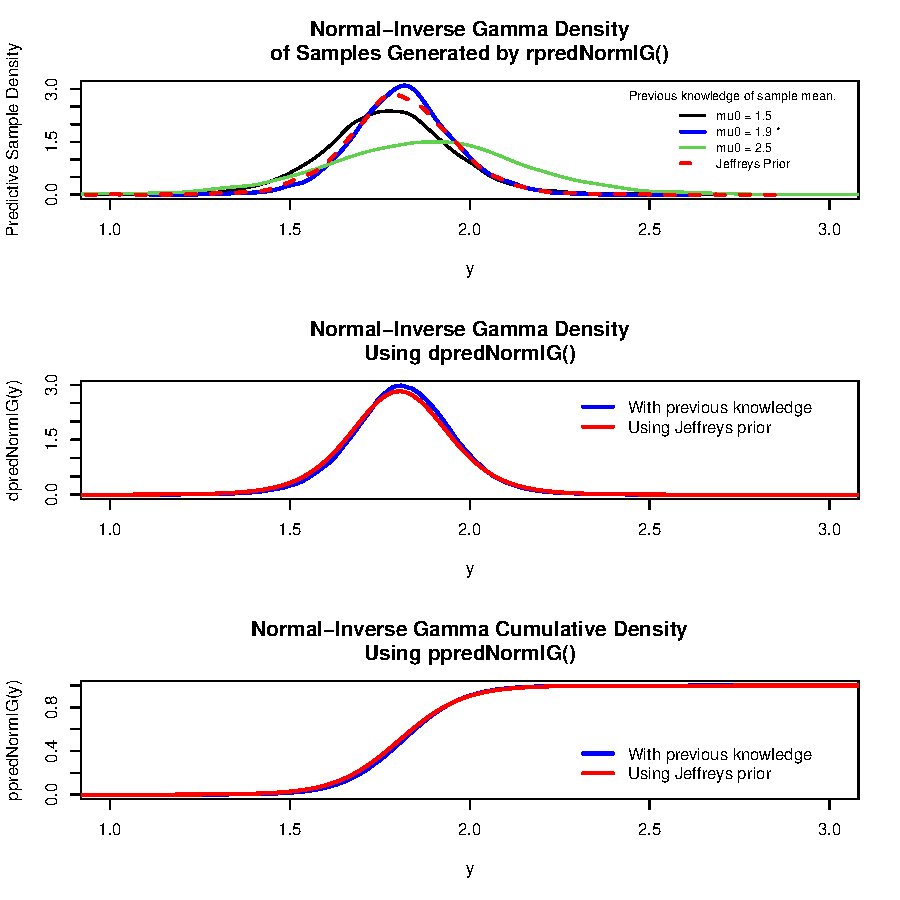
\includegraphics{Thesis-005}

        \clearpage

    \subsubsection{Two samples}
      \paragraph{Derivation}

        For a Bayesian analysis comparing two groups we use the following sampling model (Hoff p. 127):

        \begin{flalign*}
          Y_{i,1} &= \mu + \delta + \epsilon_{i,1}\\
          Y_{i,2} &= \mu - \delta + \epsilon_{i,2}\\
          \left\{\epsilon_{i,j}\right\} &\sim\text{i.i.d. normal}\left(0,\sigma^2\right).
        \end{flalign*}

        Letting $\theta_1 = \mu + \delta$ and $\theta_2 = \mu - \delta$ we see that $\delta = \left(\theta_1 - \theta_2\right)/2$ is half the population difference in means, and $\mu = \left(\theta_1 + \theta_2\right)/2$ is the pooled average.  We'll assume conjugate prior distributions

        \begin{flalign*}
          p\left(\mu,\delta,\sigma^2\right) &= p(\mu) \times p(\delta) \times p\left(\sigma^2\right)\\
          \mu &\sim \text{normal}\left(\mu_0,\gamma^2_0\right)\\
          \delta &\sim \text{normal}\left(\delta_0,\tau^2_0\right)\\
          \sigma^2 &\sim \text{inverse-gamma}\left(\nu_0/2,\nu_0\sigma^2_0/2\right),
        \end{flalign*}

\noindent where $\nu_0$ as before is the assumed prior sample size.  The full conditional distributions follow:\\

        \indent $\left\{\mu|\mathbf{y}_1,\mathbf{y}_2,\delta,\sigma^2\right\} \sim \text{normal}\left(\mu_n,\gamma^2_n\right)$, where

        \begin{flalign*}
          \mu_n &= \gamma^2_n \times \left[\dfrac{\mu_0}{\gamma^2_0} + \dfrac{\sum_{i=1}^{n_1}\left(y_{i,1}-\delta\right) + \sum_{i=1}^{n_2}\left(y_{i,2}+\delta\right)}{\sigma^2}\right]\\
          &\\
          \gamma^2_n &=\left[\dfrac{1}{\gamma^2_0} + \dfrac{\left(n_1 + n_2\right)}{\sigma^2}\right]^{-1}
        \end{flalign*}

        \indent $\left\{\delta|\mathbf{y}_1,\mathbf{y}_2,\mu,\sigma^2\right\} \sim \text{normal}\left(\delta_n,\tau^2_n\right)$, where

        \begin{flalign*}
          \delta_n &= \tau^2_n \times \left[\dfrac{\delta_0}{\tau^2_0} + \dfrac{\sum_{i=1}^{n_1}\left(y_{i,1}-\mu\right) - \sum_{i=1}^{n_2}\left(y_{i,2}-\mu\right)}{\sigma^2}\right]\\
          &\\
          \tau^2_n &=\left[\dfrac{1}{\tau^2_0} + \dfrac{\left(n_1 + n_2\right)}{\sigma^2}\right]^{-1}
        \end{flalign*}

        \indent $\left\{\sigma^2|\mathbf{y}_1,\mathbf{y}_2,\mu,\delta\right\} \sim \text{inverse-gamma}\left(\frac{\nu_n}{2},\frac{\nu_n\sigma^2_n}{2}\right)$, where

        \begin{flalign*}
          \nu_n &= \nu_0 + n_1 + n_2\\
          \\
          \nu_n\sigma^2_n &= \nu_0\sigma^2_0 + \sum_{i=1}^{n_1}\left(y_{i,1} - [\mu + \delta]\right)^2 + \sum_{i=1}^{n_2}\left(y_{i,2} - [\mu - \delta]\right)^2\\
        \end{flalign*}

      \paragraph{R Implementation}

      The standard format R function rpredNormIG2() implements a Gibbs sampler to approximate the posterior distribution $p\left(\mu,\delta,\sigma^2|\mathbf{y}_1,\mathbf{y}_2\right)$, from which to generate predictions for the two populations as follows:
      \begin{enumerate}
        \item Set initial values $\mu = \frac{\theta_1 + \theta_2}{2}$ and $\delta = \frac{\theta_1 - \theta_2}{2}$
        \item Generate a single $\sigma^2|\mathbf{y_1},\mathbf{y_2},\mu,\delta$
        \item Generate a single $\mu|\mathbf{y_1},\mathbf{y_2},\delta,\sigma^2$
        \item Generate a single $\delta|\mathbf{y_1},\mathbf{y_2},\mu,\sigma^2$
        \item Predict $\tilde{y}_1\sim \text{normal}\left(\mu+\delta,\sigma^2\right)$ and $\tilde{y}_2\sim \text{normal}\left(\mu-\delta,\sigma^2\right)$
      \end{enumerate}

      The user provides the two samples $\mathbf{y_1}$ and $\mathbf{y_2}$ along with values for $\mu_0, \sigma^2_0, \delta_0, \tau^2_0, \nu_0$, and desired prediction sample size $N$.  The function returns $N$ predictions for each population and the vectors of generated values for $\mu$, $\delta$, and $\sigma^2$.

      \paragraph{Example}

      Hoff p. 128-129 \textit{Analysis of math score data}\\
      Math score data for two schools were based on results of a national exam in the United States, standardized to produce a nationwide mean of 50 and a standard deviation of 10.  Unless the two schools were known in advance to be extremely exceptional, reasonable prior parameters can be based on this information.  For the prior distributions of $\mu$ and $\sigma^2$, we'll take $\mu_0 = 50$ and $\sigma^2_0 = 10^2 = 100$, although this latter value is likely to be an overestimate of the within-school sampling variability.  We'll make these prior distributions somewhat diffuse, with $\gamma^2_0 = 25^2 = 625$ and $\nu_0 = 1$.  For the prior distribution on $\delta$, choosing $\delta_0 = 0$ represents the prior opinion that $\theta_1 > \theta_2$ and $\theta_2 > \theta_1$ are equally probable.  Finally, since the scores are bounded between 0 and 100, half the difference between $\theta_1$ and $\theta_2$ must be less than 50 in absolute value, so a value of $\tau^2_0 = 25^2 = 625$ seems reasonably diffuse.\\\\
      The results of a call to rpredNormIG2$\left(\mathbf{y}_1,\mathbf{y}_2,\mu_0,\sigma^2_0,\delta_0,\tau^2_0,N\right)$ are summarized in the following plot.\\

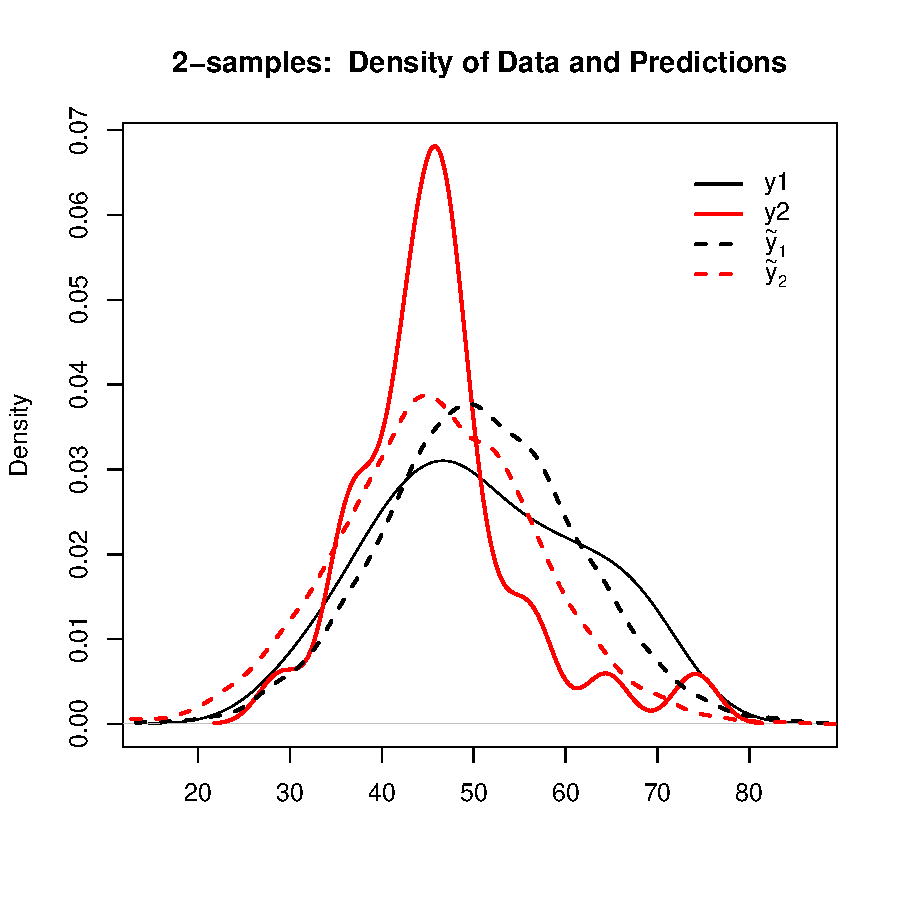
\includegraphics{Thesis-006}


    \subsubsection{$k$ samples:  Comparing multiple groups}
    For two-level data consisting of groups and units within groups, denote $y_{i,j}$ as the data on the $i$th unit in group $j$. We have the hierarchical normal model (Hoff p. 132ff):
    $$\phi_j = \left\{\theta_j,\sigma^2\right\}, p\left(y|\phi_j\right) = \text{normal}\left(\theta_j,\sigma^2\right) \text{ (within-group model)}$$
    $$\psi_j = \left\{\mu,\tau^2\right\}, p\left(\theta_j|\psi\right) = \text{normal}\left(\mu,\tau^2\right) \text{ (between-group model)}$$
    We use standard semiconjugate normal and inverse-gamma prior distributions for the fixed but unknown parameters in the model:
    \begin{flalign*}
      \sigma^2 &\sim \text{inverse-gamma}\left(\frac{\nu_0}{2},\frac{\nu_0\sigma^2_0}{2}\right)\\
      &\\
      \tau^2 &\sim \text{inverse-gamma}\left(\frac{\eta_0}{2},\frac{\eta_0\tau^2_0}{2}\right)\\
      &\\
      \mu &\sim \text{normal}\left(\mu_0,\gamma^2_0\right)\\
    \end{flalign*}

      \paragraph{Derivation}
      As with the two-sample problem, joint posterior inferences for the unknown parameters can be made by constructing a Gibbs sampler to approximate the posterior distribution $p\left(\theta_1,...,\theta_m,\mu,\tau^2,\sigma^2|\mathbf{y}_1,...,\mathbf{y}_m\right)$.  For this we need the full conditional distribution of each parameter (Hoff pp. 134-135):
      %%$$\left\{\mu|\theta_1,...,\theta_m,\tau^2\right\} \sim \text{normal}\left(\dfrac{m\bar{\theta}/\tau^2 + \mu_0/\gamma^2_0}{m/\tau^2 + 1/\gamma^2_0},\dfrac{1}{m/\tau^2+1/\gamma^2_0}\right)$$
      $$\left\{\mu|\theta_1,...,\theta_m,\tau^2\right\} \sim \text{normal}\left(\dfrac{\frac{m\bar{\theta}}{\tau^2} + \frac{\mu_0}{\gamma^2_0}}{\frac{m}{\tau^2} + \frac{1}{\gamma^2_0}},\dfrac{1}{\frac{m}{\tau^2}+\frac{1}{\gamma^2_0}}\right)$$
      $$\left\{\tau^2|\theta_1,...,\theta_m,\mu\right\} \sim \text{inverse-gamma}\left(\dfrac{\eta_0 + m}{2},\dfrac{\eta_0\tau^2_0 + \sum\left(\theta_j-\mu\right)^2}{2}\right)$$

      $$\left\{\theta_j|y_{1,j},...,y_{n,j},\sigma^2\right\} \sim \text{normal}\left(\dfrac{\frac{n_j\bar{y}_j}{\sigma^2} + \frac{1}{\tau^2}}{\frac{n_j}{\sigma^2}+\frac{1}{\tau^2}},\dfrac{1}{\frac{n_j}{\sigma^2}+\frac{1}{\tau^2}}\right)$$

      $$\left\{\sigma^2|\mathbf{\theta,y_1,...,y_n}\right\} \sim \text{inverse-gamma}\left(\dfrac{1}{2}\left[\nu_0 + \sum_{j=1}^m n_j\right],\dfrac{1}{2}\left[\nu_0\sigma^2_0 + \sum_{j=1}^m\sum_{i=1}^{n_j}\left(y_{i,j}-\theta_j\right)^2\right]\right).$$

      Note that $\sum\sum\left(y_{i,j}-\theta_j\right)^2$ is the sum of squared residuals across all groups, conditional on the within-group means, and so the conditional distribution concentrates probability around a pooled-sample estimate of the variance.


      \paragraph{R Implementation}

      The standard format R function rpredNormIGk() implements a Gibbs sampler for posterior approximation of each unknown quantity by sampling from its full conditional distribution.  From these posteriors, predictions are generated, as follows:

      \begin{enumerate}
        \item Set prior parameter values:
          \begin{flalign*}
            \nu_0,\sigma^2_0 \text{ for } p\left(\sigma^2\right)\\
            \eta_0,\tau^2_0 \text{ for } p\left(\tau^2\right)\\
            \mu_0,\gamma^2_0 \text{ for } p\left(\mu\right).
          \end{flalign*}
        \item Set initial states for the unknown parameters:
          \begin{flalign*}
            \theta_1^{(1)} &= \mathbf{\bar{y}_1},...,\theta_m^{(1)} = \mathbf{\bar{y}_m}\\
            \mu^{(1)} &= \text{mean}\left(\theta_1^{(1)},...,\theta_m^{(1)}\right)\\
            \tau^{2(1)} &= \text{var}\left(\theta_1^{(1)},...,\theta_m^{(1)}\right)\\
            \sigma^{2(1)} &= \text{mean}\left(\text{var}\left(\mathbf{y}_1\right),...,\text{var}\left(\mathbf{y}_m\right)\right))
          \end{flalign*}
        \item For $s\in\{1,...,S\}$, sample
          \begin{enumerate}
            \item $\mu^{(s+1)} \sim p\left(\mu|\theta_1^{(s)},...,\theta_m^{(s)},\tau^{2(s)}\right)$
            \item $\tau^{2(s+1)} \sim p\left(\tau^2|\theta_1^{(s)},...,\theta_m^{(s)},\mu^{(s+1)}\right)$
            \item $\sigma^{2(s+1)} \sim p\left(\sigma^2|\theta_1^{(s)},...,\theta_m^{(s)},\mathbf{y}_1,...,\mathbf{y}_m\right)$
            \item $\theta_j^{(s+1)} \sim p\left(\theta_j|\mu^{(s+1)},\tau^{2(s+1)},\sigma^{2(s+1)},\mathbf{y}_j\right)$ for $j \in \{1,...,m\}$
          \end{enumerate}
        \item For $s\in\{1,...,S\}$, generate prediction $\tilde{y}_j^{(s)} \sim \text{normal}\left(\theta_j^{(s)},\sigma^{2(s)}\right)$
      \end{enumerate}


      \paragraph{Example}
      Returning to the math scores example, data for 10th-grade students from 100 large urban schools (each having 10th-grade enrollment of at least 400) is summarized in the following plots.

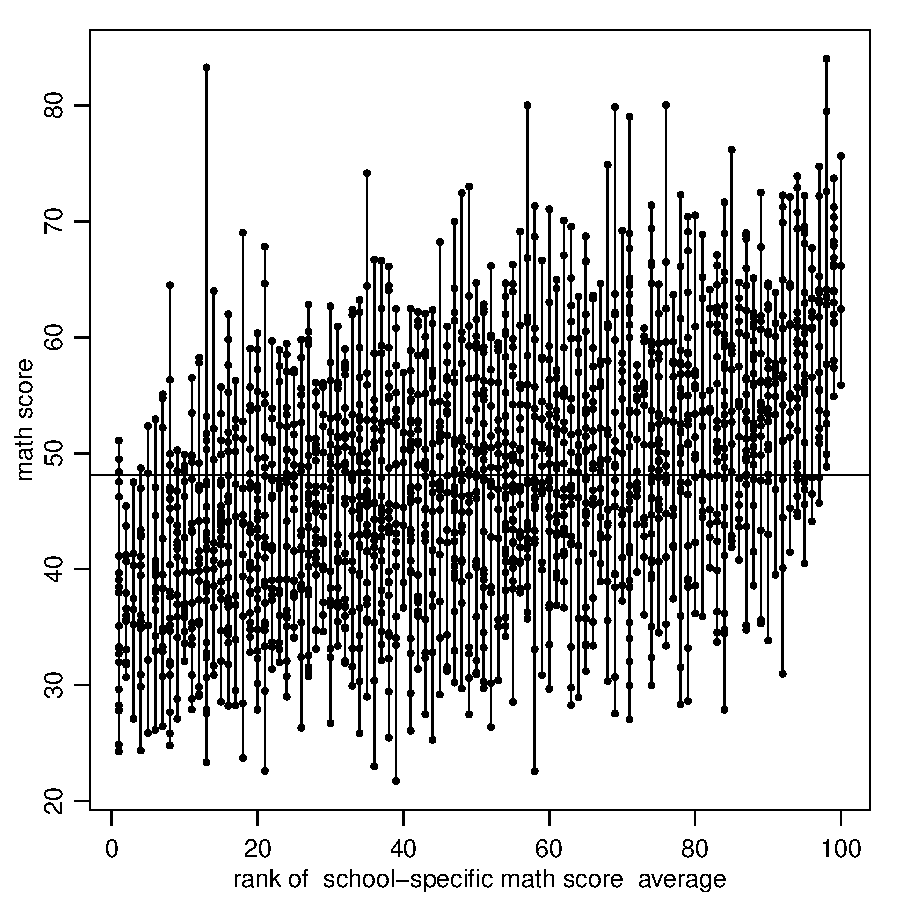
\includegraphics{Thesis-007}

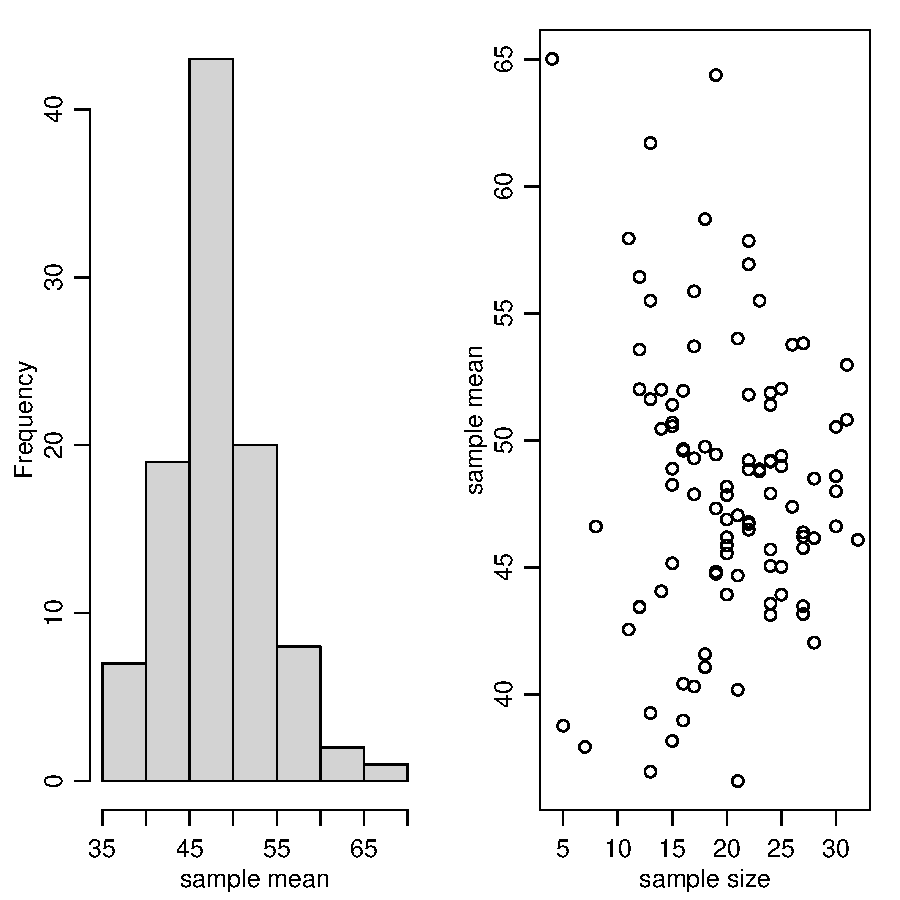
\includegraphics{Thesis-008}

      % The prior parameters that need to be specified are

      % \begin{flalign*}
      %   \left(\nu_0,\sigma^2_0\right) \text{ for } p\left(\sigma^2\right)\\
      %   \left(\eta_0,\tau^2_0\right) \text{ for } p\left(\tau^2\right)\\
      %   \left(\mu_0,\gamma^2_0\right) \text{ for } p\left(\mu\right).
      % \end{flalign*}

      % \begin{flalign*}
      %   \nu_0,\sigma^2_0 \text{ for } p\left(\sigma^2\right)\\
      %   \eta_0,\tau^2_0 \text{ for } p\left(\tau^2\right)\\
      %   \mu_0,\gamma^2_0 \text{ for } p\left(\mu\right).
      % \end{flalign*}

      For prediction, we'll use the following prior values (Hoff p. 137):

      \begin{flalign*}
        \sigma^2_0&:  100 \text{ (within-school variance)}\\
        \nu_0&:  1 \text{ (prior sample size)}\\
        \tau^2_0&:  100 \text{ (between-school variance)}\\
        \eta_0&:  1 \text{ (prior sample size)}\\
        \mu_0&:  50 \text{ (prior mean of school means)}\\
        \gamma^2_0&:  25 \text{ (prior variance of school means)}
      \end{flalign*}

\textcolor{red}{Below:  Pick a couple of schools that show different relationships between teh data and the prediction}

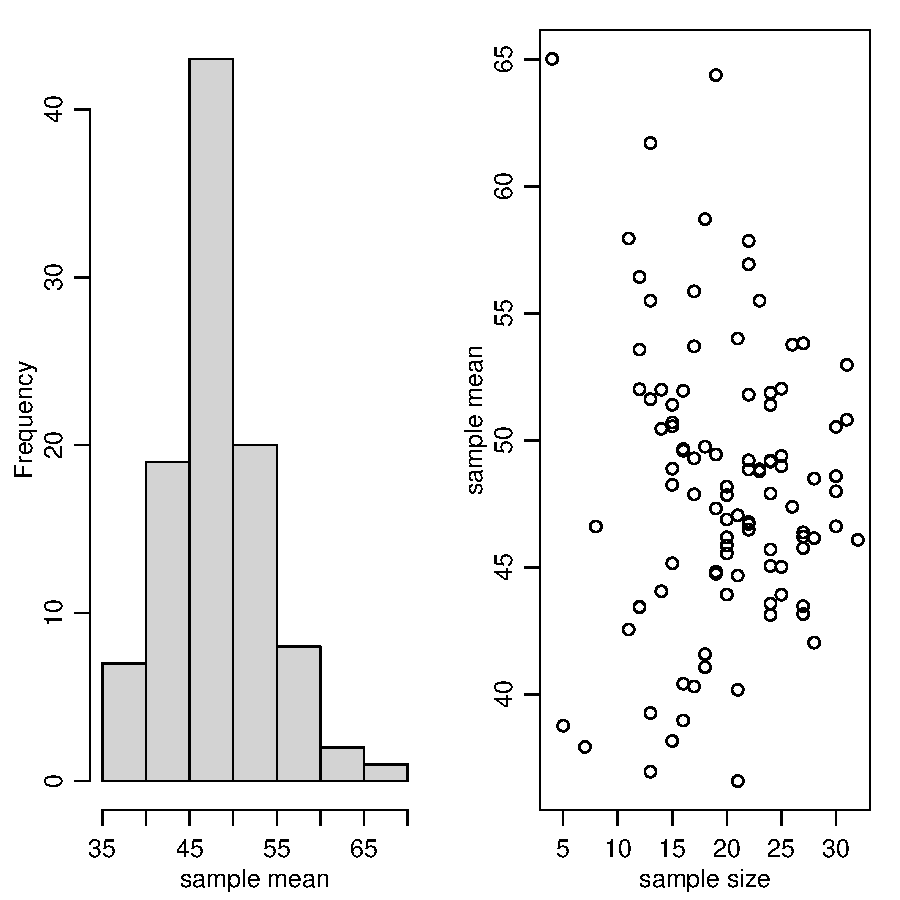
\includegraphics{Thesis-009}

      \paragraph{Ranking Treatments}

\clearpage


\section{Chapter 2:  Normal Regression with Zellner's $g$-prior}

\subsection{Least Squares Estimation with Example (Hoff p. 149ff.)}

Regression modeling is concerned with describing how the sampling istribution of one random variable $Y$ varies with another variable or set of variables $\mathbf{x} = \left(x_1,...,x_p\right)$.  Specifically, a regression model postulates a form for $p(y|\mathbf{x})$, the conditional distribution of $Y$ given $\mathbf{x}$.  Estimation of $p(y|\mathbf{x})$ is made using data $y_1,...,y_n$ that are gathered under a variety of conditions $\mathbf{x}_1,...,\mathbf{x}_n$.

The normal linear regression model specifies that, in addition to $E[Y|\mathbf{x}]$ being linear, the sampling variability around the mean is i.i.d. normal:

\begin{flalign*}
    \epsilon_1,...,\epsilon_n &\overset{\text{i.i.d}}{\sim} \text{normal}\left(0,\sigma^2\right)\\
    Y_i &= \beta^T \mathbf{x}_i + \epsilon_i
\end{flalign*}

This model provides a complete specification of the joint probability density of observed data $y_1,...,y_n$ conditional upon $\mathbf{x}_1,...,\mathbf{x}_n$ and values of $\beta$ and $\sigma^2$:

\begin{flalign}
    p\left(y_1,...y_n|\mathbf{x}_1,...,\mathbf{x}_n,\beta,\sigma^2\right) &= \prod_{i=1}^n p\left(y_i|\mathbf{x}_i,\beta,\sigma^2\right) \nonumber\\
    &= \left(2\pi\sigma^2\right)^{-n/2}\text{exp}\left\{-\frac{1}{2\sigma^2}\sum_{i=1}^n\left(y_i - \beta^T\mathbf{x}_i\right)^2\right\} \label{conditional_density}
\end{flalign}

Another way to write this joint probability density is in terms of the multivariate normal distribution:  Let $\mathbf{y}$ be the $n$-dimensional column vector $\left(y_1,...,y_n\right)^T$ and let $\mathbf{X}$ be the $n \times p$ matrix whose $i$th row is $\mathbf{x}_i = \left\{ x_{i,1}, x_{i,2}, ..., x_{i,p} \right\}$.  Then the normal regression model is

$$\{\mathbf{y}|\mathbf{X},\beta,\sigma^2\} \sim \text{multivariate normal}\left(\mathbf{X}\beta,\sigma^2\mathbf{I}\right),$$

where $\mathbf{I}$ is the $p \times p$ identity matrix and

\begin{equation*}
    \mathbf{X}\beta =
    \begin{pmatrix}
        \mathbf{x}_1 \\
        \mathbf{x}_2 \\
        \vdots  \\
        \mathbf{x}_n
    \end{pmatrix}
    \begin{pmatrix}
        \beta_1 \\
        \beta_2 \\
        \vdots \\
        \beta_p
    \end{pmatrix}
    =
    \begin{pmatrix}
        \beta_1 x_{1,1} + \cdots + \beta_p x_{1,p} \\
        \vdots \\
        \beta_1 x_{n,1} + \cdots + \beta_p x_{n,p} \\
    \end{pmatrix}
    =
    \begin{pmatrix}
        E\left[Y_1|\mathbf{\beta},\mathbf{x}_1\right] \\
        \vdots \\
        E\left[Y_n|\mathbf{\beta},\mathbf{x}_n\right] \\
    \end{pmatrix}
\end{equation*}

The density (\ref{conditional_density}) depends on $\beta$ through the residuals $\left(y_i - \beta^T\mathbf{x}_i\right)$.  We compute the ordinary least squares estimates

$$\hat{\beta}_{ols} = \left(\mathbf{X}^T\mathbf{X}\right)^{-1}\mathbf{X}^T\mathbf{y}$$

and

$$\hat{\sigma}^2_{ols} = \frac{SSR\left(\hat{\beta}_{ols}\right)}{(n-p)} = \frac{\sum\left(y_i - \hat{\beta}_{ols}^T x_i\right)^2}{(n-p)}.$$

\clearpage

\textit{Example:  Oxygen uptake (from Kuehl (2000), Hoff p. 149ff)}

Twelve healthy men who did not exercise regularly were recruited to take part in a study of the effects of two different exercise regimens on oxygen uptake.  Six of the twelve men were randomly assigned to a 12-week flat-terrain running program, and the remaining six were assigned to a 12-week step aerobics program.  The maximum oxygen uptake of each subject was measured (in liters per minute) while running on an inclined treadmill, both before and after the 12-week program.  Of interest is how a subject's change in maximal oxygen uptake may depend on which program they were assigned to.  However, other factors, such as age, are expected to affect the change in maximal uptake as well.  The results are shown here:

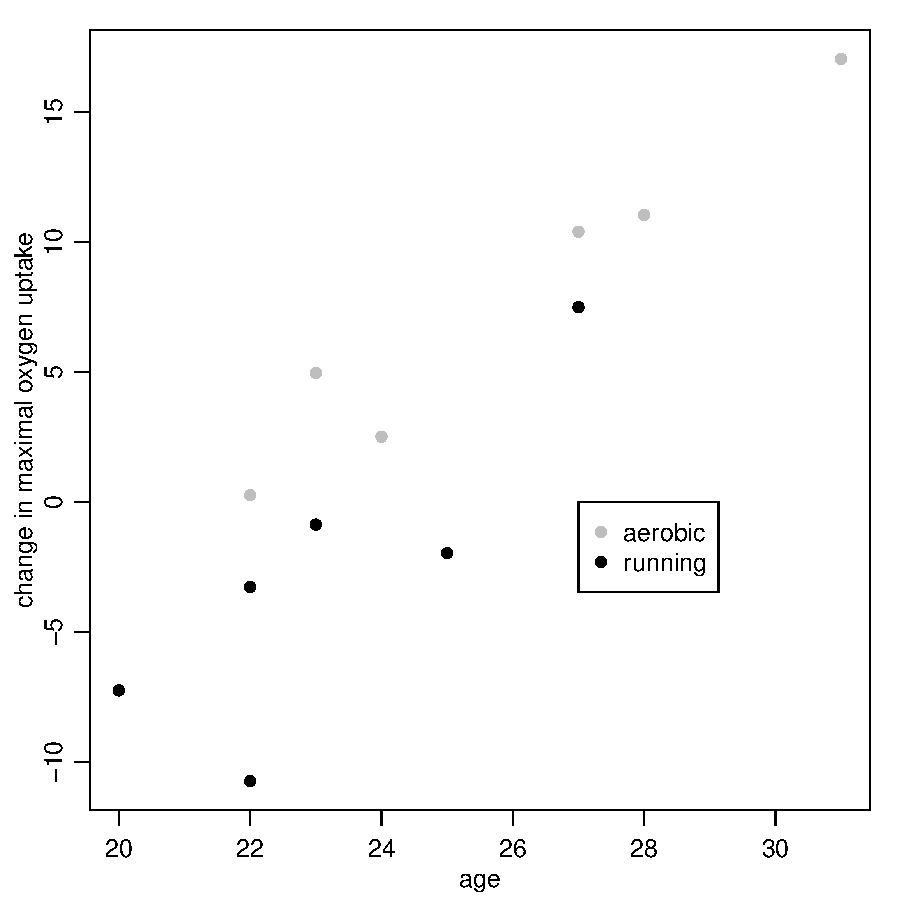
\includegraphics{Thesis-010}

Hoff's regression model:

% \begin{flalign*}
%     Y_i &= \beta_1x_{i,1} + \beta_2x_{i,2} + \beta_3x_{i,3} + \beta_4x_{i,4} + \epsilon_i, \text{ where}\\
%     x_{i,1} &= 1 \text{ for each subject } i\\
%     x_{i,2} &= 0 \text{ if subject } j \text{ is on the running program, } 1 \text{ if on aerobic}\\
%     x_{i,3} &= \text{ age of subject } i\\
%     x_{i,4} &= x_{i,2} \times x_{i,3}
% \end{flalign*}

%\begin{subequations}
    \begin{align}
        Y_i &= \beta_1x_{i,1} + \beta_2x_{i,2} + \beta_3x_{i,3} + \beta_4x_{i,4} + \epsilon_i, \text{ where} \label{example_model}\\
        x_{i,1} &= 1 \text{ for each subject } i \nonumber \\
        x_{i,2} &= 0 \text{ if subject } j \text{ is on the running program, } 1 \text{ if on aerobic} \nonumber \\
        x_{i,3} &= \text{ age of subject } i \nonumber \\
        x_{i,4} &= x_{i,2} \times x_{i,3} \nonumber
    \end{align}
%\end{subequations}

% \begin{subequations}
% \begin{align}
% \frac{\mathrm{d} x}{\mathrm{d} t} &=\sigma(y-x)\label{eqn:line-1} \\
% \frac{\mathrm{d} y}{\mathrm{d} t} &=x(\rho-z)-y\label{eqn:line-2} \\
% \frac{\mathrm{d} z}{\mathrm{d} t} &=x y-\beta z
% \end{align}
% \label{eqn:all-lines}
% \end{subequations}
%
% Look at the first line \ref{eqn:line-1}, and now look at the second line \ref{eqn:line-2}. They are both part of the whole system \ref{eqn:all-lines}.

Under this model the conditional expectations of $Y$ for the two different levels of $x_{i,1}$ are

\begin{flalign*}
    E[Y|\mathbf{x}] &= \beta_1 + \beta_3 \times \text{ age if } x_1 = 0, \text{ and}\\
    E[Y|\mathbf{x}] &= \left(\beta_1 + \beta_2\right) + \left(\beta_3 + \beta_4\right) \times \text{ age if } x_1 = 1
\end{flalign*}

In other words, the model assumes that the relationship is linear in age for both exercise groups, with the difference in intercepts given by $\beta_2$ and the difference in slopes given by $\beta_4$.  If we assumed that $\beta_2 = \beta_4 = 0$, then we would have identical lines for both groups.  If we assumed $\beta_4 =  0$ then we would have a different line for each group but they would be parallel.  Allowing all coefficients to be non-zero gives us two unrelated lines.  Some different possibilities are depicted graphically below:\\\\

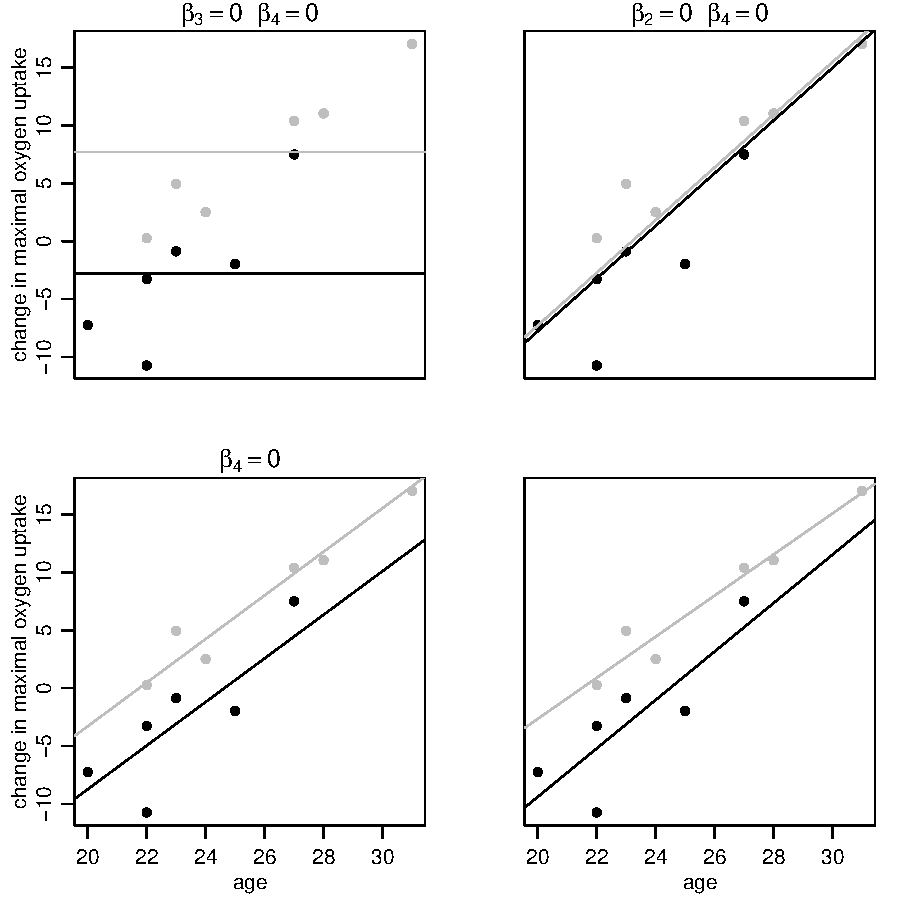
\includegraphics{Thesis-011}

Let's find the least squares regression estimates for the model in \ref{example_model}, and use the results to evaluate the differences between the two exercise groups.  The ages of the 12 subjects, along with their observed changes in maximal oxygen uptake, are

\begin{flalign*}
    \mathbf{x}_3 &= (23,22,22,25,27,20,31,23,27,28,22,24)\\
    \mathbf{y}   &= (-0.87,-10.74,-3.27,-1.97,7.50,-7.25,17.05,4.96,10.40,11.05,0.26,2.51),
\end{flalign*}

\noindent with the first six elements of each vector corresponding to the subjects in the running group and the latter six corresponding ot sujects in the aerobics group.  After constructing the $12 \time 4$ matrix $\mathbf{X}$ out of the vectors $\mathbf{x}_1,\mathbf{x}_2,\mathbf{x}_3,\mathbf{x}_4$ defined as in (\ref{example_model}), the matrices $\mathbf{X}^T\mathbf{X}$ and $\mathbf{X}^T\mathbf{y}$ can be computed, from which we get $\beta_{ols} = (-51.29,13.11,2.09,-0.32)^T$:\\



\begin{Schunk}
\begin{Sinput}
> n <- length(y)
> x1 <- rep(1,n)
> x4 <- x2*x3
> X = cbind(x1,x2,x3,x4)
> p = ncol(X)
> beta.ols<- solve(t(X)%*%X)%*%t(X)%*%y
> sig2.ols = (t(y-X%*%beta.ols)%*%(y-X%*%beta.ols)/(n-p))[1]
> sig2.ols
\end{Sinput}
\begin{Soutput}
[1] 8.542477
\end{Soutput}
\begin{Sinput}
> #sampling variance-covariance matrix of beta.ols:
> SIG2.ols = solve(t(X)%*%X)*sig2.ols
> #standard errors for the components of beta.ols:
> SE.ols = sqrt(diag(SIG2.ols))
> betadata = cbind(beta.ols,SE.ols)
> colnames(betadata) = c("beta.ols","SE.ols")
> betadata
\end{Sinput}
\begin{Soutput}
      beta.ols     SE.ols
x1 -51.2939459 12.2522126
x2  13.1070904 15.7619762
x3   2.0947027  0.5263585
x4  -0.3182438  0.6498086
\end{Soutput}
\end{Schunk}

This means that the estimated linear relationship between uptake and age has an intercept and slope of -51.29 and 2.09 for the running group, and -51.29 + 13.11 = -38.18 and 2.09 - 0.32 = 1.77 for the aerobics group.  These two lines are plotted in the fourth panel of Figure XX.  We obtain unbiased estimate $\sigma^2 = SSR(\hat{\beta}_{ols})/(n-p) = 8.54$, and use this to compute the standard error of the components of $\hat{\beta}_{ols}$, which are 12.25, 15.76, 0.53, and 0.65, respectively.  comparing the values of $\hat{\beta}_{ols}$ to their standard errors suggests that the evidence for differences between the two exercise regimens is not very strong.

\clearpage

  \subsection{Bayesian Estimation for a Regression Model (Hoff p. 154ff)}

  \subsubsection{Derivation}

    \paragraph{A semiconjugate prior distribution}
    A semiconjugate prior distribution for $\beta$ and $\sigma^2$ is used when there is information available about the parameters.  The sampling density of the data (Equation \ref{conditional_density}) is

    $$p(\mathbf{y}|\mathbf{X},\beta,\sigma^2) \propto \text{exp}\{-\frac{1}{2\sigma^2}\text{SSR}(\beta)\} = \text{exp}\{-\frac{1}{2\sigma^2}[\mathbf{y}^T\mathbf{y} - 2\beta^T\mathbf{X}^T\mathbf{y}+\beta^T\mathbf{X}^T\mathbf{X}\beta]\}.$$

    The role that $\beta$ plays in the exponent looks very similar to that played by $\mathbf{y}$, and the distribution of $\mathbf{y}$ is multivariate normal.  This suggests that a multivariate normal prior distribution for $\beta$ is conjugate:  if $\beta \sim \text{multivariate normal}(\beta_0,\Sigma_0)$, then

    \begin{flalign*}
        p&(\beta|\mathbf{y,X},\sigma^2)\\
        &\propto p(\mathbf{y}|\mathbf{X},\beta, \sigma^2) \times p(\beta)\\
        &\propto \text{exp}\{-\frac{1}{2}(-2\beta^T\mathbf{X}^T\mathbf{y}/\sigma^2 + \beta^T\mathbf{X}^T\mathbf{X}\beta/\sigma^2) - \frac{1}{2}(-2\beta^T\Sigma_0^{-1}\beta_0 + \beta^T\Sigma_0^{-1}\beta)\}\\
        &=\text{exp}\{\beta^T(\Sigma_0^{-1}\beta_0 + \mathbf{X}^T\mathbf{y}/\sigma^2) - \frac{1}{2}\beta^T(\Sigma_0^{-1} + \mathbf{X}^T\mathbf{X}/\sigma^2)\beta\}
    \end{flalign*}

    This is proportional to a multivariate normal density, with

    \begin{flalign}
        Var[\beta|\mathbf{y,X},\sigma^2] &= (\Sigma_0^{-1} + \mathbf{X}^T\mathbf{X}/\sigma^2)^{-1} \label{semiconj_var}\\
        \text{E}[\beta|\mathbf{y,X},\sigma^2] &= (\Sigma_0^{-1} + \mathbf{X}^T\mathbf{X}/\sigma^2)^{-1} (\Sigma_0^{-1}\beta_0 + \mathbf{X}^T\mathbf{y}/\sigma^2). \label{semiconj_expec}
    \end{flalign}

As usual, we can gain some understanding of these formulae by considering some limiting cases.  If the elements of the prior precision matrix $\Sigma_0^{-1}$ are small in magnitude, then the conditional expectation E$[\beta|\mathbf{y,X},\sigma^2]$ is approximately equal to $(\mathbf{X}^T\mathbf{X})^{-1}\mathbf{X}^T\mathbf{y}$, the least squares estimate. On the other hand, if the measurement precision is very small ($\sigma^2$ is very large), then the expectation is approximately $\beta_0$, the prior expectation.\\

As in most normal sampling problems, the semiconjugate prior distribution for $\sigma^2$ is an inverse-gamma distriution.  Letting $\gamma = 1/\sigma^2$ be the measurement precision, if $\gamma \sim \text{gamma}(\nu_0/2,\nu_0\sigma^2_0/2)$, then


\begin{flalign*}
    p(\gamma|\mathbf{y,X},\beta) &\propto p(\gamma)p(\mathbf{y}|\mathbf{X},\beta,\gamma)\\
        &\propto \left[\gamma^{\nu_0/2-1}\text{exp}(-\gamma \times \nu_0\sigma^2_0/2)\right] \times
                 \left[\gamma^{n/2}\text{exp}(-\gamma \times \text{SSR}(\beta)/2)\right]\\
        &= \gamma^{(\nu_0+n)/2-1} \text{exp}(-\gamma[\nu_0\sigma^2_0 + \text{SSR}(\beta)]/2),
\end{flalign*}

\noindent which we recognize as a gamma density, so that

$$\{\sigma^2|\mathbf{y,X},\beta\} \sim \text{inverse-gamma}([\nu_0 + n]/2,[\nu_0\sigma^2_0 + \text{SSR}(\beta)]/2).$$

\noindent Constructing a Gibbs sampler to approximate the joint posterior distribution $p(\beta,\sigma^2|\mathbf{y,X})$ is then straightforward:  given current values $\{\beta^{(s)},\sigma^{2(s)}\}$, new values can be generated by

\begin{enumerate}
    \item updating $\beta$:
    \begin{enumerate}
        \item compute $\mathbf{V} = \text{Var}[\beta|\mathbf{y,X},\sigma^{2(s)}]$ and $\mathbf{m} = \text{E}[\beta|\mathbf{y,X},\sigma^{2(s)}]$
        \item sample $\beta^{(s+1)} \sim \text{multivariate normal}(\mathbf{m,V})$
    \end{enumerate}
    \item updating $\sigma^2$:
    \begin{enumerate}
        \item compute SSR$(\beta^{(s+1)})$
        \item sample $\sigma^{2(s+1)} \sim \text{inverse-gamma}([\nu_0 + n]/2,[\nu_0\sigma_0^2 + \text{SSR}(\beta^{(s+1)})]/2)$.
    \end{enumerate}
\end{enumerate}

    \paragraph{Default and weakly informative prior distributions}
    In situations where prior information is unavailable or difficult to quantify, an alternative ``default" class of prior distributions is given. Specification of the prior parameters $(\beta_0, \Sigma_0)$ and $(\nu_0,\sigma^2_0)$ that represent actual prior information for a Bayesian analysis can be difficult.  For a prior distribution that is not going to represent real prior information about the parameters, we choose one that is as minimally informative as possible.  The resulting posterior distribution, then, will represent the posterior information of someone who began with little knowledge of the population being studied.  Here we will employ Zellner's ``$g$-prior" (Zellner, 1986).  We choose $\beta_0 = \mathbf{0}$ and $\Sigma_0 = k(\mathbf{X}^T\mathbf{X})^{-1}, k = g\sigma^2, g > 0$, which satisfies a desired condition that the regression parameter estimation be invariant to changes in the scale of the regressors.  With this, equations \ref{semiconj_var} and \ref{semiconj_expec} reduce to

\begin{flalign}
    \text{Var}[\beta|\mathbf{y,X},\sigma^2] &= [\mathbf{X^TX}/(g\sigma^2) + \mathbf{X^TX}/\sigma^2]^{-1} = \frac{g}{g+1}\sigma^2(\mathbf{X^TX})^{-1} \label{noninf_var}\\
    \text{E}[\beta|\mathbf{y,X},\sigma^2] &= [\mathbf{X^TX}/(g\sigma^2) + \mathbf{X^TX}/\sigma^2]^{-1}\mathbf{X^Ty}/\sigma^2 = \frac{g}{g+1}\sigma^2(\mathbf{X^TX})^{-1}\mathbf{X^Ty}.\label{noninf_expec}
\end{flalign}

Letting

$$\mathbf{V} = \frac{g}{g+1}\sigma^2(\mathbf{X^TX})^{-1} \text{ and } \mathbf{m} = \frac{g}{g+1}\sigma^2(\mathbf{X^TX})^{-1}\mathbf{X^Ty}$$

we arrive at posteriors

\begin{flalign}
    \{\sigma^2|\mathbf{y,X}\} &\sim \text{inverse-gamma}([\nu_0 + n]/2,[\nu_0\sigma^2_0 + \text{SSR}_g]/2) \label{noninf_sig2_post}\\
    \{\beta|\mathbf{y,X},\sigma^2\} &\sim \text{multivariate normal}\left(\frac{g}{g+1}\hat{\beta}_{ols},\frac{g}{g+1}\sigma^2[\mathbf{X^TX}]^{-1}\right).\label{noninf_beta_post}
\end{flalign}

Here $\text{SSR}_g = \mathbf{y^Ty - m^TV^{-1}m = y^T(I - }\frac{g}{g+1}\mathbf{X(X^TX)^{-1}X^T)y}$.\\

Simple Monte Carlo approximation can be used to sample from the joint posterior density $p(\sigma^2,\beta|\mathbf{y,X})$ as follows:

\begin{enumerate}
    \item sample $\sigma^2 \sim \text{inverse-gamma}([\nu_0 + n]/2,[\nu_0\sigma^2_0 + \text{SSR}_g]/2)$
    \item sample $\beta \sim \text{multivariate normal}\left(\frac{g}{g+1}\hat{\beta}_{ols},\frac{g}{g+1}\sigma^2[\mathbf{X^TX}]^{-1}\right)$.
\end{enumerate}

  \subsubsection{R Implementation}

The standard format R function rpredNormReg() approximates the joint posterior density $p(\sigma^2,\beta|\mathbf{y,X})$ using one of the two methods described above, as selected by the user.//

If prior information is known:



In the absence of prior information, predictions are made by means of Monte Carlo sampling:

\begin{enumerate}
    \item sample $\sigma^2 \sim \text{inverse-gamma}([\nu_0 + n]/2,[\nu_0\sigma^2_0 + \text{SSR}_g]/2)$
    \item sample $\beta \sim \text{multivariate normal}\left(\frac{g}{g+1}\hat{\beta}_{ols},\frac{g}{g+1}\sigma^2[\mathbf{X^TX}]^{-1}\right)$.
\end{enumerate}

\textcolor{red}{BIG ISSUE NEXT CHUNK IS CAUSING COMPILE TO FAIL.  wORK THROUGH WARNINGS}

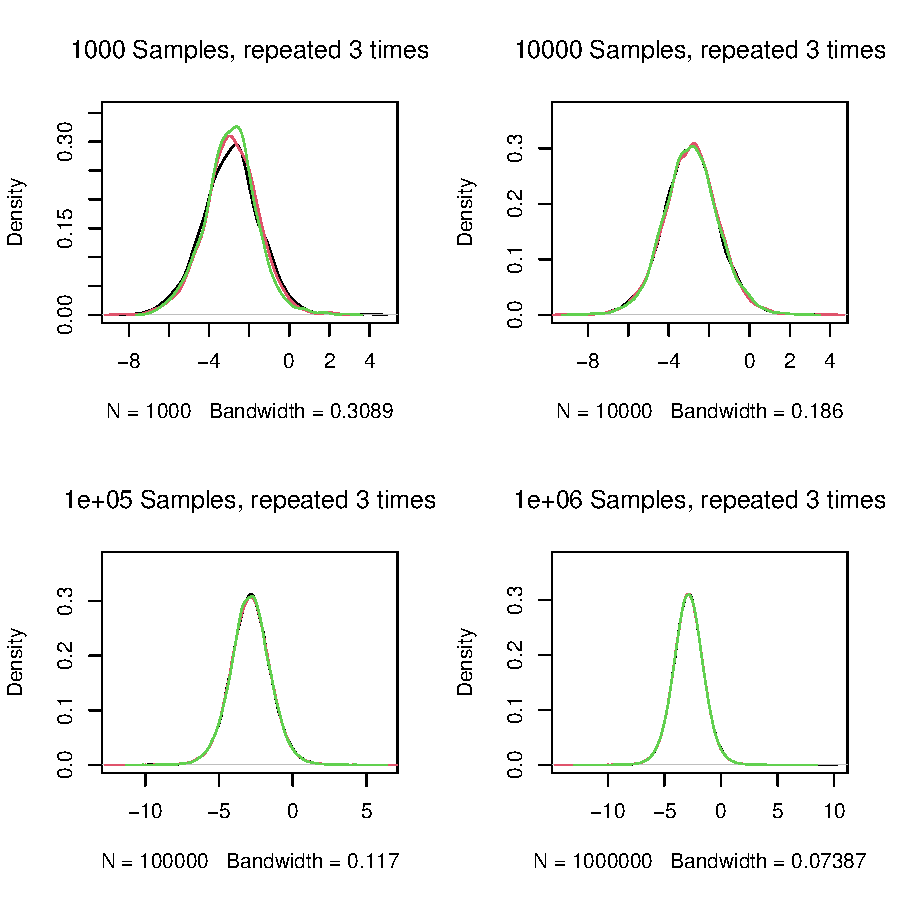
\includegraphics{Thesis-013}


%
% <<fig=TRUE,echo=FALSE>>=
% source('C:/Users/gabe/Documents/tmp/predictiveInference/R/rpredNormReg.R')
% #rpredNormReg = function(S=1,Xpred,X,y,nu0=1,s20=1,gprior = TRUE){
%
% S = 100 #desired sample size
%
% x1 <- rep(1,n)
% x2<-c(0,0,0,0,0,0,1,1,1,1,1,1)
% x3<-c(23,22,22,25,27,20,31,23,27,28,22,24)
% x4 <- x2*x3
% X = cbind(x1,x2,x3,x4)  #regression design matrix
%
% y<-c(-0.87,-10.74,-3.27,-1.97,7.50,-7.25,17.05,4.96,10.40,11.05,0.26,2.51)  #observed response vector
%
% Xpred = X[1,]           #predictor vector(s) for which prediction is desired
%
% set.seed(1)
% result = rpredNormReg(S,Xpred,X,y)
% result[1]
%
% # p = ncol(X)
% # beta.ols<- solve(t(X)%*%X)%*%t(X)%*%y
% # sig2.ols = (t(y-X%*%beta.ols)%*%(y-X%*%beta.ols)/(n-p))[1]
% @


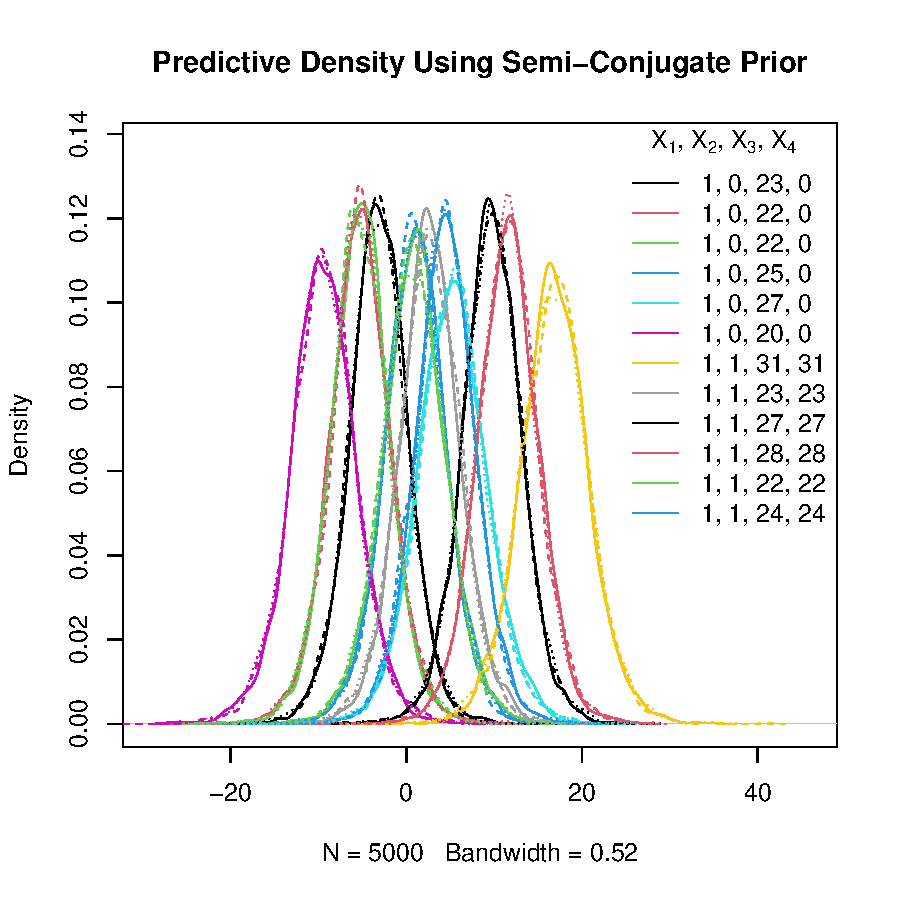
\includegraphics{Thesis-014}


  \subsubsection{Example}


\clearpage

\section{Conclusion}

\end{document}
